% ============================================================================
% Introduction to Machine Learning and Deep Learning
% Duration: 90 minutes
% ============================================================================

\documentclass[aspectratio=169,11pt]{beamer}

% ---------- Theme and colors ----------
\usecolortheme{dove}
\setbeamertemplate{navigation symbols}{}
\setbeamertemplate{footline}{%
  \hfill\usebeamerfont{page number in head/foot}%
  \usebeamercolor[fg]{normal text}%
  \insertframenumber\,/\,\inserttotalframenumber\kern1em\vskip4pt}
\setbeamerfont{frametitle}{size=\huge}

% ---------- Packages ----------
\usepackage[utf8]{inputenc}
\usepackage[T1]{fontenc}
\usepackage{amsmath,amssymb,amsfonts}
\usepackage{bm}
\usepackage{graphicx}
\usepackage{tikz}
\usetikzlibrary{shapes,arrows.meta,positioning,calc,fit,backgrounds,patterns,decorations.pathreplacing}
\usepackage{pgfplots}
\pgfplotsset{compat=1.18}
\usepackage{booktabs}
\usepackage{hyperref}
\usepackage{multicol}
\usepackage{xcolor}
\usepackage{algorithm}
\usepackage{algorithmic}

% ---------- Custom colors ----------
\definecolor{uzhblue}{rgb}{0,0,0.5}
\definecolor{uzhgreylight}{RGB}{236,238,241}
\definecolor{uzhgreydark}{RGB}{81,86,94}
\definecolor{harvardcrimson}{RGB}{153,0,0}
\definecolor{unil@blue}{RGB}{0,140,204}
\definecolor{unil@black}{RGB}{35,31,32}
\definecolor{darkgreen}{RGB}{0,100,0}
\definecolor{darkred}{RGB}{139,0,0}
\definecolor{softblue}{RGB}{70,130,180}
\definecolor{softorange}{RGB}{230,159,0}
\definecolor{softgreen}{RGB}{0,158,115}

% ---------- Set beamer colors ----------
\setbeamercolor{frametitle}{bg=uzhgreylight, fg=uzhblue}
\setbeamercolor{title}{fg=uzhblue}
\setbeamercolor{structure}{fg=uzhblue}
\setbeamercolor{block title}{bg=unil@blue, fg=white}
\setbeamercolor{block body}{bg=uzhgreylight}
\setbeamercolor{block title alerted}{bg=darkred,fg=white}
\setbeamercolor{block body alerted}{bg=red!5}
\setbeamercolor{block title example}{bg=darkgreen,fg=white}
\setbeamercolor{block body example}{bg=green!5}
\setbeamercolor{item}{fg=unil@black}
\setbeamercolor{normal text}{fg=unil@black}

% ---------- Emphasis and hyperlinks ----------
\newcommand{\emphc}[1]{\textcolor{harvardcrimson}{#1}}
\hypersetup{colorlinks,linkcolor=harvardcrimson,urlcolor=harvardcrimson}

% ---------- Math commands ----------
\newcommand{\x}{\bm{x}}
\newcommand{\w}{\bm{w}}
\newcommand{\bb}{\bm{b}}
\newcommand{\z}{\bm{z}}
\newcommand{\W}{\bm{W}}
\newcommand{\X}{\bm{X}}
\renewcommand{\a}{\bm{a}}
\newcommand{\R}{\mathbb{R}}
\newcommand{\E}[1]{\mathbb{E}\!\left[#1\right]}
\DeclareMathOperator*{\argmin}{arg\,min}
\DeclareMathOperator*{\argmax}{arg\,max}

% ---------- Title ----------
\title[Deep Learning for Dynamic Economic Models]
{Deep Learning for Economics and Finance}
\subtitle{From basic ML through DNNs to sequence models for economic time series}
\author{Simon Scheidegger}
\institute[HEC Lausanne]{HEC, University of Lausanne}
\date{}

\begin{document}

% ============================================================================
% PART 1: SETTING THE STAGE
% ============================================================================

% --- Slide 1: Title ---
{\setbeamercolor{background canvas}{bg=uzhgreylight}
\begin{frame}
\titlepage
\end{frame}
}

% --- Slide 2: Course Overview ---
\begin{frame}{Course Overview}
\footnotesize
\begin{columns}[T]
\column{0.48\textwidth}
\textbf{Block 1: Discrete-time methods}
\begin{itemize}
    \item Intro to ML \& Deep Learning
    \item Deep Equilibrium Nets (DEQNs)
    \item IRBC, NAS \& Loss Normalization
    \item OLG, Young's Method \& Sequence Space
\end{itemize}

\column{0.48\textwidth}
\textbf{Block 2: Agentic AI, continuous-time methods, applications}
\begin{itemize}
    \item Agentic Programming (AI for Research)
    \item PINNs \& CT Heterogeneous Agents (HJB+KFE)
    \item Surrogates, GPs \& Deep Kernels
    \item Climate Economics, IAMs \& Deep UQ
\end{itemize}
\end{columns}
\normalsize

\vspace{0.6cm}
\begin{center}
\textbf{All materials:}~~\url{https://github.com/sischei/Deep_Learning_for_Solving_And_Estimating_Dynamic_Economic_Models}\\[4pt]
\end{center}
\end{frame}

% --- Slide 3: Roadmap ---
\begin{frame}{Roadmap of This Lecture}
\begin{columns}[T]
\column{0.48\textwidth}
\textbf{Machine Learning Foundations}
\begin{itemize}
    \item What is ML?  Supervised, unsupervised, RL
    \item The three-step ML recipe
\end{itemize}

\vspace{0.5em}
\textbf{From Perceptrons to Deep Nets}
\begin{itemize}
    \item The perceptron and activation functions
    \item Multi-layer networks and universal approximation
\end{itemize}

\column{0.48\textwidth}
\textbf{Training, Generalization \& Practice}
\begin{itemize}
    \item Losses, gradient descent, backpropagation
    \item Regularization, optimizers, software ecosystem
\end{itemize}

\vspace{0.5em}
\textbf{Sequence Models}
\begin{itemize}
    \item RNNs, LSTMs, attention, transformers
    \item What matters for economic time series
\end{itemize}
\end{columns}
\end{frame}

% --- Learning objectives ---
\begin{frame}{Learning objectives}
\textbf{By the end of this lecture you should be able to:}
\begin{itemize}
  \item Classify supervised, unsupervised, and reinforcement learning problems and select appropriate methods for economic applications
  \item Build neural networks with multiple layers and nonlinear activations, and explain why nonlinearity is essential
  \item Implement the three-step ML recipe (model, loss, optimizer) and apply gradient descent with backpropagation
  \item Diagnose overfitting versus underfitting and apply regularization techniques to improve generalization
  \item Construct sequence models (RNNs, LSTMs, Transformers) to handle economic time series data
\end{itemize}
\end{frame}


% --- Slide 4: The Rise of Neural Networks ---
\begin{frame}{The Rise of Neural Networks}
\begin{center}
\includegraphics[width=\textwidth]{figures/rise.png}
\end{center}
\end{frame}

% --- Slide 5: AI Music Generation ---
\begin{frame}{AI Music Generation}
\begin{columns}[T]
\column{0.45\textwidth}
\begin{center}
\includegraphics[width=\textwidth]{figures/musenet.png}
\end{center}

\column{0.52\textwidth}
\textbf{OpenAI MuseNet} can generate 4-minute musical compositions with 10 different instruments, combining styles from country to Mozart to the Beatles.

\vspace{0.4cm}
Deep learning enables machines to:
\begin{itemize}
    \item Compose music in different genres
    \item Combine multiple instrumental tracks
    \item Learn long-range structure in sequences
\end{itemize}
\end{columns}
\end{frame}

% --- Slide 6: Style Transfer ---
\begin{frame}{Neural Style Transfer}
\begin{center}
\begin{columns}[c]
\column{0.32\textwidth}
\begin{center}
\includegraphics[width=\textwidth]{figures/dog1.png}\\[4pt]
{\small Content image}
\end{center}
\column{0.32\textwidth}
\begin{center}
\includegraphics[width=\textwidth]{figures/kandinsky.png}\\[4pt]
{\small Style image (Kandinsky)}
\end{center}
\column{0.32\textwidth}
\begin{center}
\includegraphics[width=\textwidth]{figures/dog2.png}\\[4pt]
{\small Result}
\end{center}
\end{columns}
\end{center}

\vspace{0.3cm}
{\small Gatys, Ecker \& Bethge (2015): a neural network separates and recombines content and style of images.}
\end{frame}

% --- Slide 7: Self-Driving Cars ---
\begin{frame}{Self-Driving Cars}
\begin{columns}[T]
\column{0.48\textwidth}
\begin{center}
\includegraphics[width=\textwidth]{figures/alvinn.png}\\[4pt]
{\small \textbf{ALVINN} (1989), one of the first autonomous vehicles, using a simple neural network.}
\end{center}

\column{0.48\textwidth}
\begin{center}
\includegraphics[width=\textwidth]{figures/waymo.png}\\[4pt]
{\small \textbf{Waymo} (2017+), deep learning for perception, prediction, and planning.}
\end{center}
\end{columns}
\end{frame}

% --- Slide 8: Two-Legged Robots ---
\begin{frame}{Two-Legged Robots}
\begin{columns}[T]
\column{0.48\textwidth}
\begin{center}
\includegraphics[width=0.9\textwidth]{figures/atlas.png}\\[4pt]
{\small \textbf{Boston Dynamics Atlas}\\
\url{https://www.bostondynamics.com/atlas}}
\end{center}

\column{0.48\textwidth}
\begin{center}
\includegraphics[width=0.9\textwidth]{figures/terminator.png}\\[4pt]
{\small Science fiction meets reality, deep reinforcement learning enables humanoid locomotion.}
\end{center}
\end{columns}
\end{frame}

% --- Slide 9: Coloring Old Movies ---
\begin{frame}{Coloring Old Movies}
\begin{columns}[T]
\column{0.48\textwidth}
\begin{center}
\includegraphics[width=\textwidth]{figures/bw.png}\\[4pt]
{\small Original black-and-white frame}
\end{center}

\column{0.48\textwidth}
\begin{center}
\includegraphics[width=\textwidth]{figures/color.png}\\[4pt]
{\small Automatic colorization using deep learning}
\end{center}
\end{columns}

\vspace{0.3cm}
{\small Deep neural networks learn to predict plausible colors from grayscale input, trained on millions of color images.}
\end{frame}

% --- Slide 10: A Timeline of Deep Learning ---
\begin{frame}{A Timeline of Deep Learning}
\begin{center}
\includegraphics[width=\textwidth]{figures/timeline.png}
\end{center}
\end{frame}

% --- Deep Learning in Economics and Finance ---
\begin{frame}[shrink=8]{Deep Learning in Economics and Finance}
\small
\begin{columns}[T]
\column{0.48\textwidth}
\textbf{Forecasting \& Nowcasting}
\begin{itemize}\setlength{\itemsep}{1pt}
    \item GDP nowcasting from high-frequency data
    \item Inflation forecasting with nonlinear models
    \item Yield curve modeling and term structure
\end{itemize}

\vspace{0.2cm}
\textbf{Text \& Communication}
\begin{itemize}\setlength{\itemsep}{1pt}
    \item NLP on central bank minutes and speeches
    \item Sentiment analysis of financial news
    \item Measuring policy uncertainty
\end{itemize}

\column{0.48\textwidth}
\textbf{Financial Stability \& Supervision}
\begin{itemize}\setlength{\itemsep}{1pt}
    \item Fraud and anomaly detection
    \item Credit risk scoring
    \item Stress testing and scenario generation
\end{itemize}

\vspace{0.2cm}
\textbf{Structural Models}
\begin{itemize}\setlength{\itemsep}{1pt}
    \item Solving and estimating structural models (DSGE, OLG, heterogeneous agents)
    \item Overcoming the curse of dimensionality
    \item NN-based surrogates for equilibrium computation
\end{itemize}
\end{columns}

\vspace{0.2cm}
\begin{center}
{\footnotesize \emphc{This course} focuses on the last category, using deep learning as a computational tool for economic modeling.}
\end{center}
\end{frame}

% --- Slide 11: Useful Materials ---
\begin{frame}[shrink=8]{Useful Materials}
\begin{columns}[T]
\column{0.42\textwidth}
\begin{center}
\includegraphics[width=0.9\textwidth]{figures/books1.png}
\end{center}

\column{0.55\textwidth}
\begin{enumerate}
    \item \textbf{I.\ Goodfellow, Y.\ Bengio, A.\ Courville} (2016).
          \textit{Deep Learning}. MIT Press.
          \hfill \url{https://www.deeplearningbook.org}

    \vspace{0.3cm}
    \item \textbf{K.\ P.\ Murphy} (2022).
          \textit{Probabilistic Machine Learning: An Introduction}. MIT Press.

    \vspace{0.3cm}
    \item \textbf{G.\ James et al.} (2021).
          \textit{An Introduction to Statistical Learning} (ISLR). Springer.
          \hfill \url{https://www.statlearning.com}
\end{enumerate}
\end{columns}
\end{frame}

% --- Slide 12: Why Deep Learning Now? ---
\begin{frame}[shrink=15]{Why Deep Learning Now?}
Neural networks date back to the 1940s.  Three developments made them practical:

\vspace{0.4cm}
\begin{center}
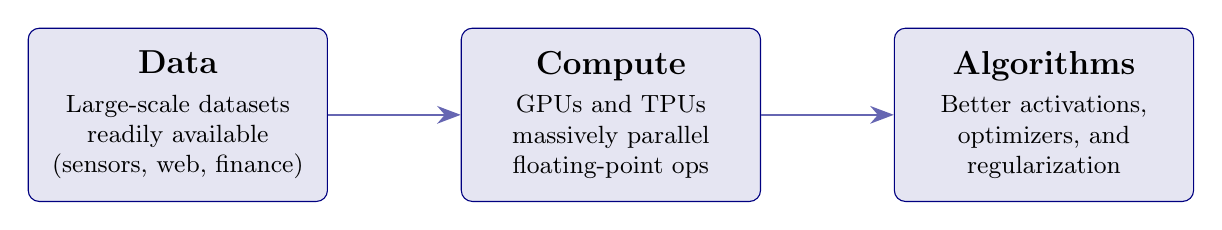
\begin{tikzpicture}[
    box/.style={rectangle, draw=uzhblue, fill=uzhblue!10, rounded corners=4pt,
                minimum width=3.8cm, minimum height=2.2cm, align=center, font=\small},
    arr/.style={-{Stealth[length=3mm]}, thick, uzhblue!60}
]
    \node[box] (data) at (0,0) {\textbf{\large Data}\\[3pt]Large-scale datasets\\readily available\\(sensors, web, finance)};
    \node[box] (hw) at (5.5,0) {\textbf{\large Compute}\\[3pt]GPUs and TPUs\\massively parallel\\floating-point ops};
    \node[box] (sw) at (11,0) {\textbf{\large Algorithms}\\[3pt]Better activations,\\optimizers, and\\regularization};

    \draw[arr] (data) -- (hw);
    \draw[arr] (hw) -- (sw);
\end{tikzpicture}
\end{center}

\vspace{0.3cm}
{\small Key milestones: Perceptron (1958), Backpropagation (1986), Deep CNN (1995), AlexNet (2012), Transformers (2017), ChatGPT (2022).}
\end{frame}


% ============================================================================
% PART 2: MACHINE LEARNING FOUNDATIONS
% ============================================================================

\section{Machine Learning Foundations}

% --- Section Divider ---
\begin{frame}{}
\begin{center}
{\Huge \textcolor{uzhblue}{Part I}}\\[0.8em]
{\LARGE Machine Learning Foundations}
\end{center}
\end{frame}

% --- Slide 7: What is Machine Learning? ---
\begin{frame}{What is Machine Learning?}
\begin{columns}[T]
\column{0.45\textwidth}
\begin{center}
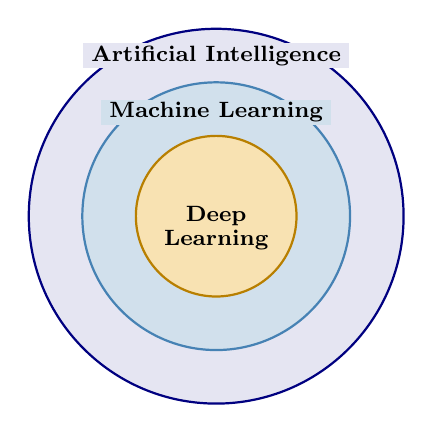
\begin{tikzpicture}[scale=0.85]
    % Concentric circles: AI > ML > DL
    \fill[uzhblue!10] (0,0) circle (2.8cm);
    \fill[softblue!25] (0,0) circle (2.0cm);
    \fill[softorange!30] (0,0) circle (1.2cm);
    \draw[uzhblue, thick] (0,0) circle (2.8cm);
    \draw[softblue, thick] (0,0) circle (2.0cm);
    \draw[softorange!80!black, thick] (0,0) circle (1.2cm);
    \node[font=\footnotesize\bfseries] at (0,0) {Deep};
    \node[font=\footnotesize\bfseries] at (0,-0.35) {Learning};
    \node[font=\footnotesize\bfseries, fill=softblue!25, inner xsep=3pt, inner ysep=1pt] at (0,1.55) {Machine Learning};
    \node[font=\footnotesize\bfseries, fill=uzhblue!10, inner xsep=3pt, inner ysep=1pt] at (0,2.4) {Artificial Intelligence};
\end{tikzpicture}
\end{center}

\column{0.52\textwidth}
\textbf{Classical programming:}

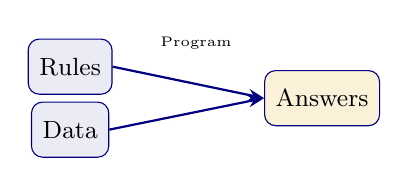
\begin{tikzpicture}[
    box/.style={rectangle, draw=uzhblue, fill=uzhblue!8, rounded corners,
                minimum height=7mm, font=\small, inner sep=4pt},
    arr/.style={-{Stealth[length=2mm]}, thick, uzhblue}]
    \node[box] (r) at (0,0) {Rules};
    \node[box] (d) at (0,-0.8) {Data};
    \node[box, fill=softorange!15] (a) at (3.2,-0.4) {Answers};
    \draw[arr] (r.east) -- (a.west);
    \draw[arr] (d.east) -- (a.west);
    \node[font=\tiny, above] at (1.6, 0.1) {Program};
\end{tikzpicture}

\vspace{0.4cm}
\textbf{Machine learning:}

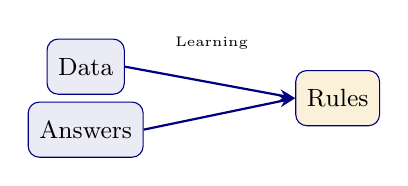
\begin{tikzpicture}[
    box/.style={rectangle, draw=uzhblue, fill=uzhblue!8, rounded corners,
                minimum height=7mm, font=\small, inner sep=4pt},
    arr/.style={-{Stealth[length=2mm]}, thick, uzhblue}]
    \node[box] (d) at (0,0) {Data};
    \node[box] (a) at (0,-0.8) {Answers};
    \node[box, fill=softorange!15] (r) at (3.2,-0.4) {Rules};
    \draw[arr] (d.east) -- (r.west);
    \draw[arr] (a.east) -- (r.west);
    \node[font=\tiny, above] at (1.6, 0.1) {Learning};
\end{tikzpicture}
\end{columns}
\end{frame}

% --- Slide 8: Types of ML ---
\begin{frame}{Types of Machine Learning}
\begin{columns}[T]
\column{0.32\textwidth}
\begin{block}{\centering Supervised}
    Given labeled pairs $\{(\x^{(i)}, y^{(i)})\}_{i=1}^{m}$, learn a mapping $h:\mathcal{X}\to\mathcal{Y}$.

    \vspace{0.3em}
    \textbf{Regression:} $y\in\R$\\
    \textbf{Classification:} $y\in\{0,1,\dots,K\}$
\end{block}

\column{0.32\textwidth}
\begin{block}{\centering Unsupervised}
    Given only $\{\x^{(i)}\}_{i=1}^{m}$, discover hidden structure.

    \vspace{0.3em}
    \textbf{Clustering:} group similar points\\
    \textbf{Dim.\ reduction:} compress features
\end{block}

\column{0.32\textwidth}
\begin{block}{\centering Reinforcement}
    An agent acts in an environment, receives rewards, and learns a policy $\pi$.

    \vspace{0.3em}
    \textbf{Policy:} $a_t = \pi(s_t)$\\
    \textbf{Goal:} maximize $\sum_t \gamma^t r_t$
\end{block}
\end{columns}

\vspace{0.5cm}
\begin{center}
{\small This course covers \textbf{both} paradigms: we begin with the \emph{supervised} pipeline (model, loss, optimizer)\\
and then build on it for the \emph{self-supervised residual} methods at the heart of the course (DEQNs, PINNs).}
\end{center}
\end{frame}

% --- Slide 9: Supervised Regression ---
\begin{frame}{Supervised Learning: Regression}
\begin{columns}[T]
\column{0.52\textwidth}
\textbf{Goal:} predict a continuous target $y\in\R$ from features $\x\in\R^d$.

\vspace{0.3cm}
\textbf{Setup:}
\begin{itemize}
    \item Training data: $\{(\x^{(i)}, y^{(i)})\}_{i=1}^{m}$
    \item Model (hypothesis): $\hat{y} = h(\x;\bm{\theta})$
    \item Parameters $\bm{\theta}$ learned from data
\end{itemize}

\vspace{0.3cm}
\textbf{Linear example:}
\[
    h_{\bm{\theta}}(x) = \theta_0 + \theta_1 x
\]

\column{0.45\textwidth}
\begin{center}
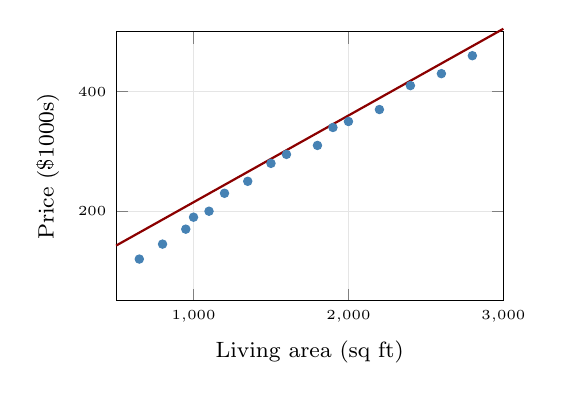
\begin{tikzpicture}
\begin{axis}[
    width=6.5cm, height=5cm,
    xlabel={Living area (sq ft)},
    ylabel={Price (\$1000s)},
    xlabel style={font=\footnotesize},
    ylabel style={font=\footnotesize},
    tick label style={font=\tiny},
    xmin=500, xmax=3000, ymin=50, ymax=500,
    grid=major, grid style={gray!20},
    clip=false
]
    % Scatter data
    \addplot[only marks, mark=*, mark size=1.5pt, softblue] coordinates {
        (650,120) (800,145) (950,170) (1000,190) (1100,200) (1200,230)
        (1350,250) (1500,280) (1600,295) (1800,310) (1900,340)
        (2000,350) (2200,370) (2400,410) (2600,430) (2800,460)
    };
    % Regression line
    \addplot[thick, darkred, domain=500:3000, samples=2]{70 + 0.145*x};
\end{axis}
\end{tikzpicture}
\end{center}
\end{columns}
\end{frame}

% --- Slide 10: Classification ---
\begin{frame}{Supervised Learning: Classification}
\begin{columns}[T]
\column{0.50\textwidth}
\textbf{Goal:} assign an input $\x$ to one of $K$ classes.

\vspace{0.3cm}
\textbf{Example -- Credit scoring:}
\begin{itemize}
    \item Features: income, savings
    \item Labels: low-risk / high-risk
    \item Decision boundary separates classes
\end{itemize}

\vspace{0.3cm}
A simple linear rule:
\[
    \text{if } \w^\top \x + b > 0 \;\Rightarrow\; \text{low-risk}
\]

\column{0.47\textwidth}
\begin{center}
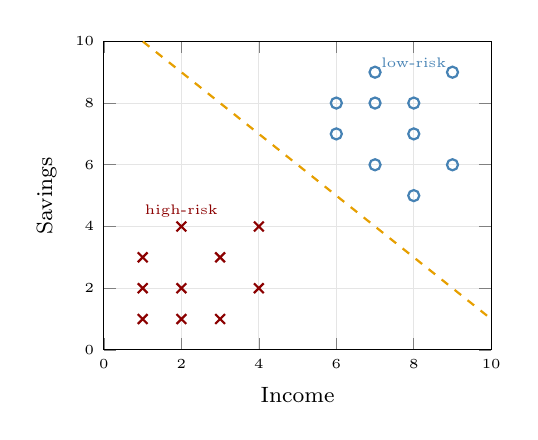
\begin{tikzpicture}
\begin{axis}[
    width=6.5cm, height=5.5cm,
    xlabel={Income}, ylabel={Savings},
    xlabel style={font=\footnotesize},
    ylabel style={font=\footnotesize},
    tick label style={font=\tiny},
    xmin=0, xmax=10, ymin=0, ymax=10,
    grid=major, grid style={gray!20},
]
    % Low-risk (blue)
    \addplot[only marks, mark=o, mark size=2pt, softblue, thick] coordinates {
        (6,7) (7,6) (8,5) (7,8) (8,7) (9,6) (6,8) (8,8) (9,9) (7,9)
    };
    % High-risk (red)
    \addplot[only marks, mark=x, mark size=2.5pt, darkred, thick] coordinates {
        (1,2) (2,1) (3,3) (2,4) (1,3) (4,2) (3,1) (2,2) (4,4) (1,1)
    };
    % Decision boundary
    \addplot[thick, softorange, dashed, domain=0:10, samples=2]{11-x};
    \node[font=\tiny, softblue] at (axis cs:8,9.3) {low-risk};
    \node[font=\tiny, darkred] at (axis cs:2,4.5) {high-risk};
\end{axis}
\end{tikzpicture}
\end{center}
\end{columns}
\end{frame}

% --- Slide 11: The ML Recipe ---
\begin{frame}{The Machine Learning Recipe}
Every machine learning algorithm follows the same three steps:

\vspace{0.5cm}
\begin{center}
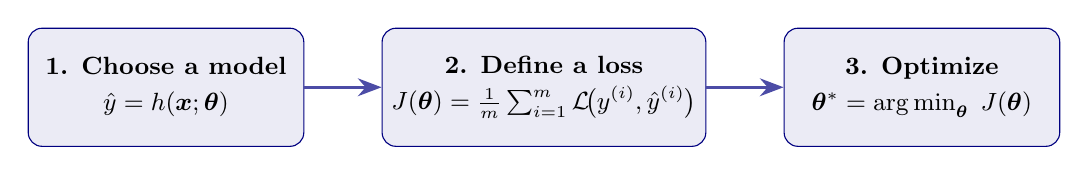
\begin{tikzpicture}[
    mlstep/.style={rectangle, draw=uzhblue, fill=uzhblue!8, rounded corners=5pt,
                 minimum width=3.5cm, minimum height=1.5cm, align=center, font=\small},
    arr/.style={-{Stealth[length=3mm]}, very thick, uzhblue!70}
]
    \node[mlstep] (m) at (0,0) {\textbf{1. Choose a model}\\[2pt]$\hat{y} = h(\x;\bm{\theta})$};
    \node[mlstep] (l) at (4.8,0) {\textbf{2. Define a loss}\\[2pt]$J(\bm{\theta}) = \frac{1}{m}\sum_{i=1}^{m}\mathcal{L}\!\big(y^{(i)},\hat{y}^{(i)}\big)$};
    \node[mlstep] (o) at (9.6,0) {\textbf{3. Optimize}\\[2pt]$\bm{\theta}^{*} = \argmin_{\bm{\theta}}\; J(\bm{\theta})$};

    \draw[arr] (m) -- (l);
    \draw[arr] (l) -- (o);
\end{tikzpicture}
\end{center}

\vspace{0.3cm}
\begin{block}{Cost function example (supervised regression: Mean Squared Error)}
\[
    J(\bm{\theta}) \;=\; \frac{1}{m}\sum_{i=1}^{m}\!\big(h_{\bm{\theta}}(\x^{(i)}) - y^{(i)}\big)^{2}
\]
\end{block}
{\footnotesize\emphc{Same recipe, different loss.}  DEQNs and PINNs (later chapters) replace step~2 by an Euler-equation or PDE residual; steps~1 and~3 are unchanged.}
\end{frame}

% --- Slide 12: Supervised Learning Pipeline ---
\begin{frame}{Supervised Learning Pipeline}
\begin{center}
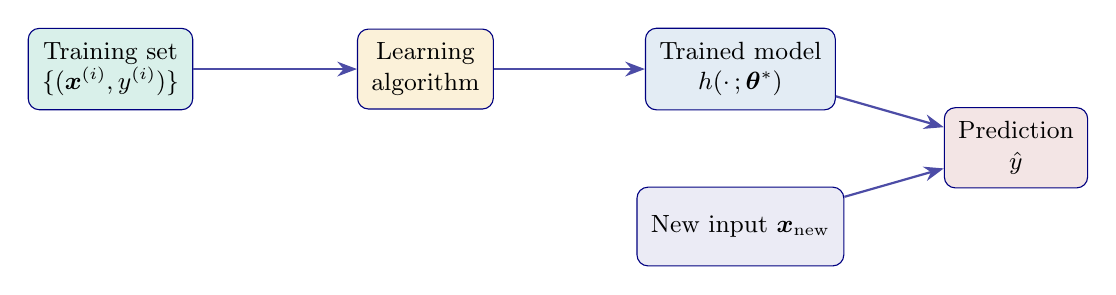
\begin{tikzpicture}[
    box/.style={rectangle, draw=uzhblue, fill=uzhblue!8, rounded corners=4pt,
                minimum height=1cm, align=center, font=\small, inner sep=5pt},
    arr/.style={-{Stealth[length=2.5mm]}, thick, uzhblue!70}
]
    \node[box, fill=softgreen!15] (data) at (0,0) {Training set\\$\{(\x^{(i)}, y^{(i)})\}$};
    \node[box, fill=softorange!15] (algo) at (4,0) {Learning\\algorithm};
    \node[box, fill=softblue!15] (model) at (8,0) {Trained model\\$h(\cdot\,;\bm{\theta}^{*})$};
    \node[box] (xnew) at (8,-2) {New input $\x_{\mathrm{new}}$};
    \node[box, fill=darkred!10] (pred) at (11.5,-1) {Prediction\\$\hat{y}$};

    \draw[arr] (data) -- (algo);
    \draw[arr] (algo) -- (model);
    \draw[arr] (model) -- (pred);
    \draw[arr] (xnew) -- (pred);
\end{tikzpicture}
\end{center}

\vspace{0.5cm}
\textbf{Computationally, we need:}
\begin{itemize}
    \item Data (labeled examples)
    \item Linear algebra and automatic differentiation
    \item An optimization routine (gradient-based)
\end{itemize}
\end{frame}

% --- Slide 13: Unsupervised Learning ---
\begin{frame}{Unsupervised Learning}
\begin{columns}[T]
\column{0.50\textwidth}
No labels, only inputs $\{\x^{(i)}\}_{i=1}^{m}$. The goal is to discover hidden structure.

\vspace{0.3cm}
\textbf{Clustering:} partition data into groups of similar points (e.g., customer segmentation, image compression).

\vspace{0.3cm}
\textbf{Dimensionality reduction:} project high-dimensional data to a lower-dimensional space (e.g., PCA, autoencoders).

\column{0.47\textwidth}
\begin{center}
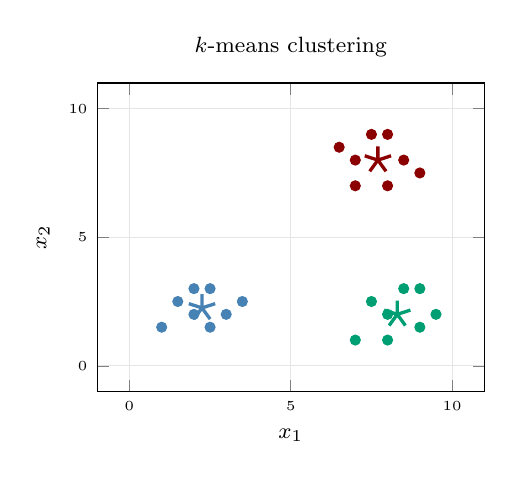
\begin{tikzpicture}
\begin{axis}[
    width=6.5cm, height=5.5cm,
    xlabel={$x_1$}, ylabel={$x_2$},
    xlabel style={font=\footnotesize},
    ylabel style={font=\footnotesize},
    tick label style={font=\tiny},
    xmin=-1, xmax=11, ymin=-1, ymax=11,
    grid=major, grid style={gray!20},
    title={\footnotesize $k$-means clustering},
    title style={font=\footnotesize},
]
    % Cluster 1 (blue)
    \addplot[only marks, mark=*, mark size=1.8pt, softblue] coordinates {
        (2,2) (2.5,1.5) (1.5,2.5) (3,2) (2,3) (1,1.5) (2.5,3) (3.5,2.5)
    };
    % Cluster 2 (red)
    \addplot[only marks, mark=*, mark size=1.8pt, darkred] coordinates {
        (7,8) (8,7) (7.5,9) (8.5,8) (9,7.5) (7,7) (8,9) (6.5,8.5)
    };
    % Cluster 3 (green)
    \addplot[only marks, mark=*, mark size=1.8pt, softgreen] coordinates {
        (8,2) (9,1.5) (7.5,2.5) (8.5,3) (9.5,2) (7,1) (8,1) (9,3)
    };
    % Centroids
    \addplot[only marks, mark=star, mark size=5pt, softblue, very thick] coordinates {(2.25,2.25)};
    \addplot[only marks, mark=star, mark size=5pt, darkred, very thick] coordinates {(7.7,8)};
    \addplot[only marks, mark=star, mark size=5pt, softgreen, very thick] coordinates {(8.3,2)};
\end{axis}
\end{tikzpicture}
\end{center}
\end{columns}
\end{frame}

% --- Slide 14: Reinforcement Learning ---
\begin{frame}{Reinforcement Learning (Brief)}
\begin{center}
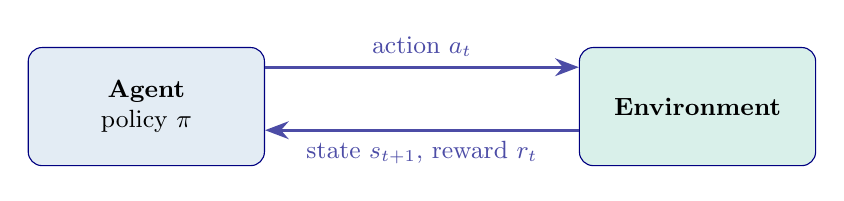
\begin{tikzpicture}[
    box/.style={rectangle, draw=uzhblue, fill=uzhblue!8, rounded corners=5pt,
                minimum width=3cm, minimum height=1.5cm, align=center, font=\small},
    arr/.style={-{Stealth[length=3mm]}, very thick, uzhblue!70}
]
    \node[box, fill=softblue!15] (agent) at (0,0) {\textbf{Agent}\\policy $\pi$};
    \node[box, fill=softgreen!15] (env) at (7,0) {\textbf{Environment}};

    \draw[arr] ([yshift=5mm]agent.east) -- node[above, font=\small]{action $a_t$} ([yshift=5mm]env.west);
    \draw[arr] ([yshift=-3mm]env.west) -- node[below, font=\small]{state $s_{t+1}$, reward $r_t$} ([yshift=-3mm]agent.east);
\end{tikzpicture}
\end{center}

\vspace{0.5cm}
\begin{itemize}
    \item The agent learns a policy $\pi(a\mid s)$ to maximize cumulative discounted reward $\sum_{t=0}^{\infty}\gamma^t r_t$.
    \item No explicit supervision, only delayed reward signals.
    \item Applications: game playing (AlphaGo), robotics, portfolio optimization.
\end{itemize}

\vspace{0.3cm}
{\small We will not cover RL in this course, but the neural network tools you learn here are the building blocks for deep RL. Deep RL for sequential decision-making shares the Bellman structure developed in Chapters~2--5.}
\end{frame}

% ============================================================================
% PART 3: FROM PERCEPTRONS TO DEEP NETWORKS
% ============================================================================

\section{Artificial Neural Networks}

% --- Section Divider ---
\begin{frame}{}
\begin{columns}[c]
\column{0.65\textwidth}
\begin{center}
{\Huge \textcolor{uzhblue}{Part II}}\\[0.8em]
{\LARGE From Perceptrons to Deep Networks}
\end{center}
\column{0.30\textwidth}
\begin{center}
\includegraphics[width=0.7\textwidth]{figures/r2d2.png}
\end{center}
\end{columns}
\end{frame}

% --- Biological Neurons ---
\begin{frame}[shrink=8]{Biological Neurons}
\begin{columns}[T]
\column{0.55\textwidth}
\begin{center}
\includegraphics[width=\textwidth]{figures/neurons.png}
\end{center}

\column{0.42\textwidth}
\textbf{The brain} is a massively parallel computer made of $\sim$86 billion neurons.

\vspace{0.3cm}
Each neuron:
\begin{itemize}
    \item Receives signals via \textbf{dendrites}
    \item Integrates signals in the \textbf{cell body}
    \item Transmits output along the \textbf{axon}
    \item Communicates at \textbf{synapses}
\end{itemize}

\vspace{0.3cm}
{\small Artificial neural networks are a \textit{very loose} abstraction of this biological architecture.}
\end{columns}
\end{frame}

% --- Slide 16: McCulloch-Pitts Neuron ---
\begin{frame}{The Artificial Neuron (McCulloch \& Pitts, 1943)}
{\small\emphc{From biology to math:} turn the neuron on the previous slide into an equation, synapses become weights $w_i$, dendritic inputs become $x_i$, the soma's integration becomes a sum, and firing becomes a nonlinear activation.}
\vspace{0.2cm}
\begin{columns}[T]
\column{0.55\textwidth}
\begin{center}
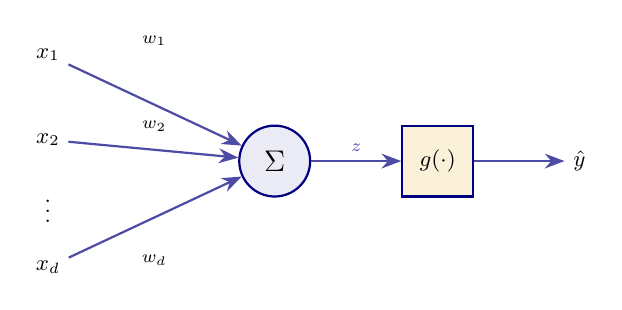
\begin{tikzpicture}[scale=0.9, transform shape,
    neuron/.style={circle, draw=uzhblue, thick, minimum size=10mm, fill=uzhblue!8},
    arr/.style={-{Stealth[length=2.5mm]}, thick, uzhblue!70}]

    % Inputs
    \node[font=\small] (x1) at (0,2) {$x_1$};
    \node[font=\small] (x2) at (0,0.8) {$x_2$};
    \node[font=\small] at (0,-0.1) {$\vdots$};
    \node[font=\small] (xm) at (0,-1) {$x_d$};

    % Weights
    \node[font=\scriptsize, above] at (1.5,2) {$w_1$};
    \node[font=\scriptsize, above] at (1.5,0.8) {$w_2$};
    \node[font=\scriptsize, below] at (1.5,-0.7) {$w_d$};

    % Sum node
    \node[neuron, font=\large] (sum) at (3.2,0.5) {$\Sigma$};

    % Activation
    \node[rectangle, draw=uzhblue, thick, fill=softorange!15,
          minimum width=10mm, minimum height=10mm, font=\small] (act) at (5.5,0.5) {$g(\cdot)$};

    % Output
    \node[font=\small] (out) at (7.5,0.5) {$\hat{y}$};

    % Arrows
    \draw[arr] (x1) -- (sum);
    \draw[arr] (x2) -- (sum);
    \draw[arr] (xm) -- (sum);
    \draw[arr] (sum) -- node[above, font=\scriptsize]{$z$} (act);
    \draw[arr] (act) -- (out);
\end{tikzpicture}
\end{center}

\column{0.42\textwidth}
Three components:
\begin{enumerate}
    \item \textbf{Weighted inputs} $w_i$ (synaptic weights)
    \item \textbf{Summation:} $z = \sum_{j=1}^{d} w_j x_j$
    \item \textbf{Activation} $g(z)$: nonlinear function determining whether the neuron ``fires''
\end{enumerate}

\vspace{0.3cm}
{\small Original model used a step function as activation. Modern networks use smooth alternatives.}
\end{columns}
\end{frame}

% --- Hebb's Rule ---
\begin{frame}[shrink=10]{Hebb's Rule (1949)}
{\small\emphc{The missing ingredient --- learning:} the McCulloch--Pitts neuron is static; its weights $w_i$ are fixed by hand. Hebb asks \textit{how should the weights change with experience?}}
\vspace{0.2cm}
\begin{columns}[T]
\column{0.55\textwidth}
\textbf{``Neurons that fire together, wire together.''}

\vspace{0.3cm}
Donald Hebb proposed that if neuron $A$ repeatedly causes neuron $B$ to fire, the synapse from $A$ to $B$ is strengthened:
\[
    \Delta w_{ij} = \eta\, x_i\, y_j
\]

\vspace{0.3cm}
This is the foundation of learning rules in artificial neural networks.

\vspace{0.3cm}
{\small Analogy: every time you eat chocolate and feel happy, the association between ``chocolate'' and ``happiness'' neurons strengthens!}

\column{0.40\textwidth}
\begin{center}
\includegraphics[width=\textwidth]{figures/chocolate.png}
\end{center}
\end{columns}
\end{frame}

% --- Slide 17: The Perceptron ---
\begin{frame}{The Perceptron}
\begin{columns}[T]
\column{0.48\textwidth}
\begin{center}
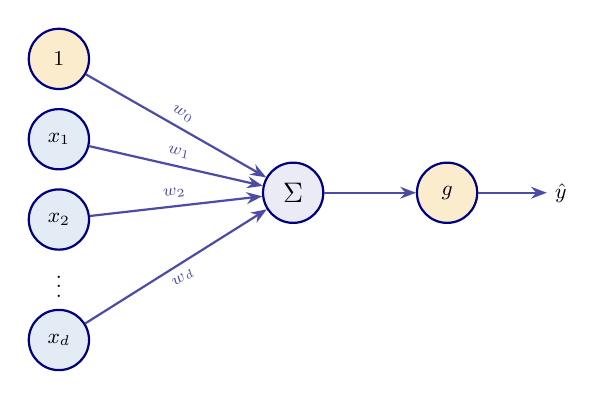
\begin{tikzpicture}[scale=0.85, transform shape,
    neuron/.style={circle, draw=uzhblue, thick, minimum size=9mm, fill=uzhblue!8},
    arr/.style={-{Stealth[length=2mm]}, thick, uzhblue!70}]

    % Bias
    \node[neuron, fill=softorange!20, font=\small] (b) at (0,3) {$1$};
    \node[neuron, fill=softblue!15, font=\small] (x1) at (0,1.8) {$x_1$};
    \node[neuron, fill=softblue!15, font=\small] (x2) at (0,0.6) {$x_2$};
    \node[font=\small] at (0,-0.3) {$\vdots$};
    \node[neuron, fill=softblue!15, font=\small] (xd) at (0,-1.2) {$x_d$};

    % Sum
    \node[neuron, font=\large] (sum) at (3.5,1) {$\Sigma$};

    % Activation
    \node[neuron, fill=softorange!20, font=\small] (act) at (5.8,1) {$g$};

    % Output
    \node[font=\small] (out) at (7.5,1) {$\hat{y}$};

    % Weight labels
    \draw[arr] (b) -- node[above, font=\scriptsize, sloped]{$w_0$} (sum);
    \draw[arr] (x1) -- node[above, font=\scriptsize, sloped]{$w_1$} (sum);
    \draw[arr] (x2) -- node[above, font=\scriptsize, sloped]{$w_2$} (sum);
    \draw[arr] (xd) -- node[below, font=\scriptsize, sloped]{$w_d$} (sum);
    \draw[arr] (sum) -- (act);
    \draw[arr] (act) -- (out);
\end{tikzpicture}
\end{center}

\column{0.48\textwidth}
\textbf{Forward pass:}
\[
    \hat{y} \;=\; g\!\left(w_0 + \sum_{j=1}^{d} x_j\, w_j\right)
\]

In vector notation, with $\w = (w_1,\dots,w_d)^\top$:
\[
    \hat{y} \;=\; g\!\big(w_0 + \x^\top \w\big)
\]

\vspace{0.2cm}
\begin{itemize}
    \item $w_0$ is the \textbf{bias} (shifts activation)
    \item $g(\cdot)$ is a nonlinear \textbf{activation function}
\end{itemize}
\end{columns}
\end{frame}

% --- Slide 18: Forward Propagation Vector Form ---
\begin{frame}{Forward Propagation -- Vector Form}
Absorbing the bias into the weight vector, define
$\tilde{\x} = (1, x_1, \dots, x_d)^\top \in \R^{d+1}$ and
$\tilde{\w} = (w_0, w_1, \dots, w_d)^\top \in \R^{d+1}$. Then:
\[
    \boxed{\hat{y} \;=\; g\!\big(\tilde{\x}^\top \tilde{\w}\big)}
\]

\vspace{0.5cm}
\begin{block}{Key insight}
The perceptron computes a \textbf{weighted linear combination} of its inputs, applies a \textbf{nonlinearity}, and produces a scalar output.  Without $g$, this is just linear regression.
\end{block}

\vspace{0.3cm}
{\small We will use the notation $z = \w^\top\x + b$ (separating bias $b$ from weights $\w$) for the remainder of this lecture.}
\end{frame}

% --- Slide 19: Activation Functions ---
\begin{frame}{Activation Functions}
\begin{center}
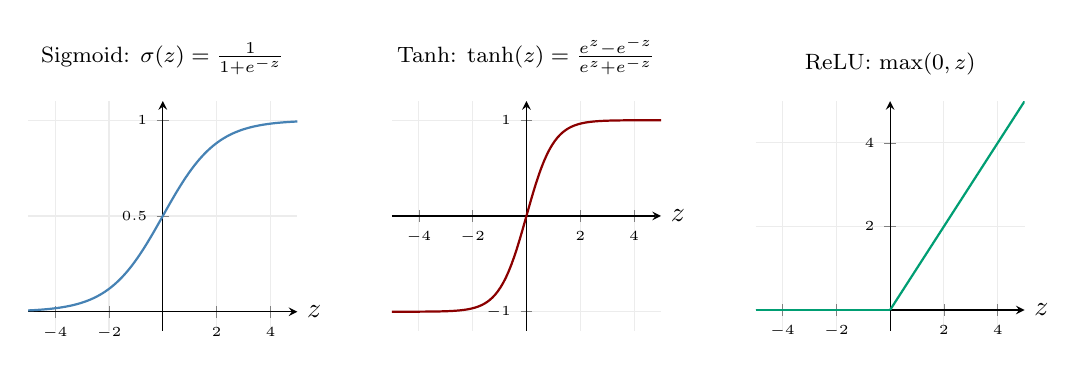
\begin{tikzpicture}
\begin{axis}[
    name=plot1,
    width=5cm, height=4.5cm,
    title={\footnotesize Sigmoid: $\sigma(z) = \frac{1}{1+e^{-z}}$},
    title style={font=\footnotesize},
    xlabel={$z$}, xlabel style={font=\tiny},
    tick label style={font=\tiny},
    xmin=-5, xmax=5, ymin=-0.1, ymax=1.1,
    grid=major, grid style={gray!15},
    axis lines=middle,
    every axis x label/.style={at={(current axis.right of origin)}, anchor=west},
    every axis y label/.style={at={(current axis.above origin)}, anchor=south},
]
    \addplot[thick, softblue, domain=-5:5, samples=100]{1/(1+exp(-x))};
\end{axis}

\begin{axis}[
    at={($(plot1.east)+(1.2cm,0)$)}, anchor=west,
    name=plot2,
    width=5cm, height=4.5cm,
    title={\footnotesize Tanh: $\tanh(z) = \frac{e^z - e^{-z}}{e^z + e^{-z}}$},
    title style={font=\footnotesize},
    xlabel={$z$}, xlabel style={font=\tiny},
    tick label style={font=\tiny},
    xmin=-5, xmax=5, ymin=-1.2, ymax=1.2,
    grid=major, grid style={gray!15},
    axis lines=middle,
    every axis x label/.style={at={(current axis.right of origin)}, anchor=west},
    every axis y label/.style={at={(current axis.above origin)}, anchor=south},
]
    \addplot[thick, darkred, domain=-5:5, samples=100]{tanh(x)};
\end{axis}

\begin{axis}[
    at={($(plot2.east)+(1.2cm,0)$)}, anchor=west,
    width=5cm, height=4.5cm,
    title={\footnotesize ReLU: $\max(0, z)$},
    title style={font=\footnotesize},
    xlabel={$z$}, xlabel style={font=\tiny},
    tick label style={font=\tiny},
    xmin=-5, xmax=5, ymin=-0.5, ymax=5,
    grid=major, grid style={gray!15},
    axis lines=middle,
    every axis x label/.style={at={(current axis.right of origin)}, anchor=west},
    every axis y label/.style={at={(current axis.above origin)}, anchor=south},
]
    \addplot[thick, softgreen, domain=-5:0, samples=2]{0};
    \addplot[thick, softgreen, domain=0:5, samples=2]{x};
\end{axis}
\end{tikzpicture}
\end{center}

\vspace{-0.1cm}
\begin{center}
\begin{small}
\begin{tabular}{lccc}
\toprule
& \textbf{Sigmoid} & \textbf{Tanh} & \textbf{ReLU} \\
\midrule
Range & $(0,1)$ & $(-1,1)$ & $[0,\infty)$ \\
$g'(z)$ & $\sigma(z)(1-\sigma(z))$ & $1 - \tanh^2(z)$ & $\begin{cases}1&z>0\\0&z<0\end{cases}$ \\
\bottomrule
\end{tabular}
\end{small}
\end{center}
\end{frame}

% --- Slide 20: Why Nonlinearity? ---
\begin{frame}{Why Nonlinearity Matters}
\begin{columns}[T]
\column{0.47\textwidth}
\begin{center}
{\small\textbf{Linear activation} $\Rightarrow$ linear boundary}
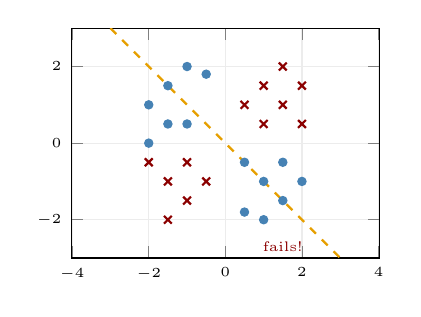
\begin{tikzpicture}
\begin{axis}[
    width=5.5cm, height=4.5cm,
    tick label style={font=\tiny},
    xmin=-3, xmax=3, ymin=-3, ymax=3,
    grid=major, grid style={gray!15},
    axis equal,
]
    % Two spirals (simplified as overlapping clusters)
    \addplot[only marks, mark=*, mark size=1.5pt, softblue] coordinates {
        (-2,1) (-1.5,1.5) (-1,2) (-0.5,1.8) (-1.5,0.5) (-2,0) (-1,0.5)
        (0.5,-1.8) (1,-2) (1.5,-1.5) (2,-1) (1.5,-0.5) (1,-1) (0.5,-0.5)
    };
    \addplot[only marks, mark=x, mark size=2pt, darkred, thick] coordinates {
        (1,1.5) (1.5,1) (2,0.5) (1.5,2) (0.5,1) (1,0.5) (2,1.5)
        (-1,-1.5) (-1.5,-1) (-2,-0.5) (-1.5,-2) (-0.5,-1) (-1,-0.5)
    };
    % Linear boundary (fails)
    \addplot[thick, softorange, dashed, domain=-3:3]{-x};
    \node[font=\tiny, darkred] at (axis cs:1.5,-2.7) {fails!};
\end{axis}
\end{tikzpicture}
\end{center}

\column{0.47\textwidth}
\begin{center}
{\small\textbf{Nonlinear activation} $\Rightarrow$ curved boundary}
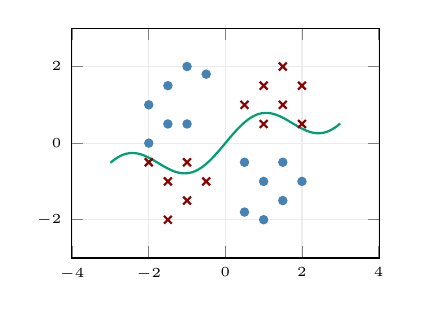
\begin{tikzpicture}
\begin{axis}[
    width=5.5cm, height=4.5cm,
    tick label style={font=\tiny},
    xmin=-3, xmax=3, ymin=-3, ymax=3,
    grid=major, grid style={gray!15},
    axis equal,
]
    \addplot[only marks, mark=*, mark size=1.5pt, softblue] coordinates {
        (-2,1) (-1.5,1.5) (-1,2) (-0.5,1.8) (-1.5,0.5) (-2,0) (-1,0.5)
        (0.5,-1.8) (1,-2) (1.5,-1.5) (2,-1) (1.5,-0.5) (1,-1) (0.5,-0.5)
    };
    \addplot[only marks, mark=x, mark size=2pt, darkred, thick] coordinates {
        (1,1.5) (1.5,1) (2,0.5) (1.5,2) (0.5,1) (1,0.5) (2,1.5)
        (-1,-1.5) (-1.5,-1) (-2,-0.5) (-1.5,-2) (-0.5,-1) (-1,-0.5)
    };
    % Nonlinear boundary
    \addplot[thick, softgreen, domain=-3:3, samples=100]{0.5*sin(deg(x*1.8))+0.3*x};
\end{axis}
\end{tikzpicture}
\end{center}
\end{columns}

\vspace{0.4cm}
\begin{alertblock}{Mathematical reason}
A composition of linear maps is still linear: $\W_2(\W_1\x+\bb_1)+\bb_2 = \W_2\W_1\x + (\W_2\bb_1+\bb_2)$.
Without nonlinearities, depth is useless.
\end{alertblock}
\end{frame}

% --- Slide 21: Perceptron Example ---
\begin{frame}{Perceptron -- A Worked Example}
\begin{columns}[T]
\column{0.50\textwidth}
Suppose we have trained weights $w_0=1$, $\w=(3, -2)^\top$, and sigmoid activation $\sigma$.

\vspace{0.3cm}
\textbf{Output:}
\[
    \hat{y} = \sigma(w_0 + \x^\top\w) = \sigma(1 + 3x_1 - 2x_2)
\]

For a new point $\x = (-1, 2)^\top$:
\begin{align*}
    z &= 1 + 3\cdot(-1) - 2\cdot 2 = -6 \\
    \hat{y} &= \sigma(-6) \approx 0.0025
\end{align*}

The discriminant line $1+3x_1-2x_2=0$ separates the two classes.

\column{0.47\textwidth}
\begin{center}
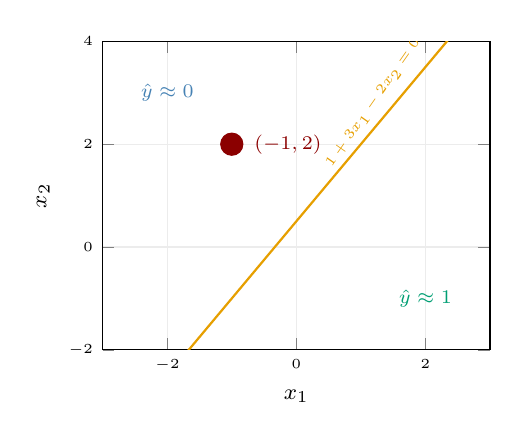
\begin{tikzpicture}
\begin{axis}[
    width=6.5cm, height=5.5cm,
    xlabel={$x_1$}, ylabel={$x_2$},
    xlabel style={font=\footnotesize},
    ylabel style={font=\footnotesize},
    tick label style={font=\tiny},
    xmin=-3, xmax=3, ymin=-2, ymax=4,
    grid=major, grid style={gray!15},
]
    % Decision boundary: 1 + 3x1 - 2x2 = 0 => x2 = 0.5 + 1.5*x1
    \addplot[thick, softorange, domain=-3:3, samples=2]{0.5 + 1.5*x};
    % New point
    \addplot[only marks, mark=*, mark size=4pt, darkred] coordinates {(-1,2)};
    \node[font=\scriptsize, darkred, right] at (axis cs:-0.8,2) {$(-1,2)$};
    % Region labels
    \node[font=\scriptsize, softblue] at (axis cs:-2,3) {$\hat{y} \approx 0$};
    \node[font=\scriptsize, softgreen] at (axis cs:2,-1) {$\hat{y} \approx 1$};
    % Boundary label
    \node[font=\tiny, softorange, rotate=55] at (axis cs:1.2,2.8) {$1+3x_1-2x_2=0$};
\end{axis}
\end{tikzpicture}
\end{center}
\end{columns}
\end{frame}

% --- Slide 22: Multi-Output Perceptron ---
\begin{frame}[shrink=15]{Multi-Output Perceptron}
\begin{columns}[T]
\column{0.50\textwidth}
\begin{center}
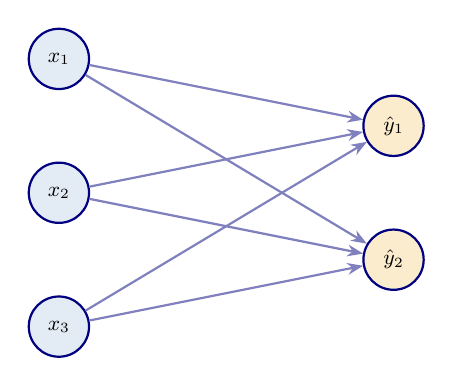
\begin{tikzpicture}[scale=0.85, transform shape,
    neuron/.style={circle, draw=uzhblue, thick, minimum size=9mm, fill=uzhblue!8},
    arr/.style={-{Stealth[length=2mm]}, thick, uzhblue!50}]

    % Inputs
    \node[neuron, fill=softblue!15, font=\small] (x1) at (0,2) {$x_1$};
    \node[neuron, fill=softblue!15, font=\small] (x2) at (0,0) {$x_2$};
    \node[neuron, fill=softblue!15, font=\small] (x3) at (0,-2) {$x_3$};

    % Outputs
    \node[neuron, fill=softorange!20, font=\small] (y1) at (5,1) {$\hat{y}_1$};
    \node[neuron, fill=softorange!20, font=\small] (y2) at (5,-1) {$\hat{y}_2$};

    % Connections
    \foreach \i in {x1,x2,x3} {
        \foreach \j in {y1,y2} {
            \draw[arr] (\i) -- (\j);
        }
    }
\end{tikzpicture}
\end{center}

\column{0.47\textwidth}
Each output unit computes its own weighted sum:
\[
    z_k = b_k + \sum_{j=1}^{d} w_{jk}\, x_j, \quad k=1,\dots,K
\]

In matrix form:
\[
    \z = \W\x + \bb, \qquad \hat{\bm{y}} = g(\z)
\]

where $\W\in\R^{K\times d}$ (one row per output unit) and $\bb\in\R^{K}$.  The same row-per-output convention is used in every later layer of this deck, so the formula extends directly to deep networks (slides 23--24).

\vspace{0.3cm}
{\small Each output has its own set of weights but shares the same inputs.}
\end{columns}
\end{frame}

% --- Slide 23: Single Hidden Layer ---
\begin{frame}{Single Hidden Layer Network}
\begin{columns}[T]
\column{0.48\textwidth}
\begin{center}
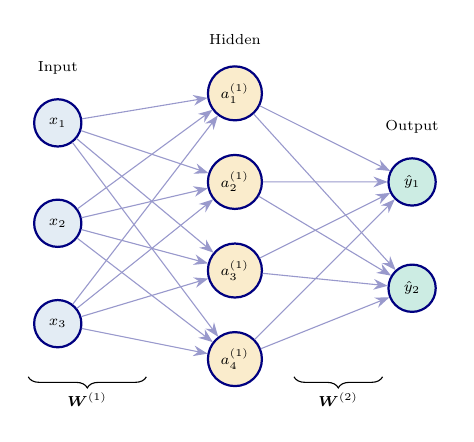
\begin{tikzpicture}[scale=0.75, transform shape,
    neuron/.style={circle, draw=uzhblue, thick, minimum size=8mm},
    arr/.style={-{Stealth[length=1.8mm]}, uzhblue!40}]

    % Input layer
    \node[neuron, fill=softblue!15, font=\scriptsize] (x1) at (0,2.5) {$x_1$};
    \node[neuron, fill=softblue!15, font=\scriptsize] (x2) at (0,0.8) {$x_2$};
    \node[neuron, fill=softblue!15, font=\scriptsize] (x3) at (0,-0.9) {$x_3$};

    % Hidden layer
    \node[neuron, fill=softorange!20, font=\scriptsize] (h1) at (3,3) {$a_1^{(1)}$};
    \node[neuron, fill=softorange!20, font=\scriptsize] (h2) at (3,1.5) {$a_2^{(1)}$};
    \node[neuron, fill=softorange!20, font=\scriptsize] (h3) at (3,0) {$a_3^{(1)}$};
    \node[neuron, fill=softorange!20, font=\scriptsize] (h4) at (3,-1.5) {$a_4^{(1)}$};

    % Output layer
    \node[neuron, fill=softgreen!20, font=\scriptsize] (y1) at (6,1.5) {$\hat{y}_1$};
    \node[neuron, fill=softgreen!20, font=\scriptsize] (y2) at (6,-0.3) {$\hat{y}_2$};

    % Connections
    \foreach \i in {x1,x2,x3} {
        \foreach \j in {h1,h2,h3,h4} { \draw[arr] (\i) -- (\j); }
    }
    \foreach \i in {h1,h2,h3,h4} {
        \foreach \j in {y1,y2} { \draw[arr] (\i) -- (\j); }
    }

    % Labels
    \node[font=\scriptsize, above] at (0,3.2) {Input};
    \node[font=\scriptsize, above] at (3,3.7) {Hidden};
    \node[font=\scriptsize, above] at (6,2.2) {Output};

    % Weight labels
    \draw[decorate, decoration={brace, amplitude=4pt, mirror}] (-0.5,-1.8) -- (1.5,-1.8)
        node[midway, below=4pt, font=\scriptsize]{$\W^{(1)}$};
    \draw[decorate, decoration={brace, amplitude=4pt, mirror}] (4,-1.8) -- (5.5,-1.8)
        node[midway, below=4pt, font=\scriptsize]{$\W^{(2)}$};
\end{tikzpicture}
\end{center}

\column{0.48\textwidth}
\textbf{Hidden layer:}
\begin{align*}
    \z^{(1)} &= \W^{(1)}\x + \bb^{(1)} \\
    \a^{(1)} &= g\!\big(\z^{(1)}\big)
\end{align*}

\textbf{Output layer:}
\begin{align*}
    \z^{(2)} &= \W^{(2)}\a^{(1)} + \bb^{(2)} \\
    \hat{\bm{y}} &= g_{\text{out}}\!\big(\z^{(2)}\big)
\end{align*}

where $\W^{(1)}\in\R^{n_1\times d}$, $\W^{(2)}\in\R^{K\times n_1}$.

\vspace{0.3cm}
{\small The hidden layer creates a \textbf{learned representation} of the input that the output layer then uses for prediction.}
\end{columns}
\end{frame}

% --- Slide 24: Deep Feedforward Network ---
\begin{frame}[shrink=8]{Deep Feedforward Networks}
\begin{center}
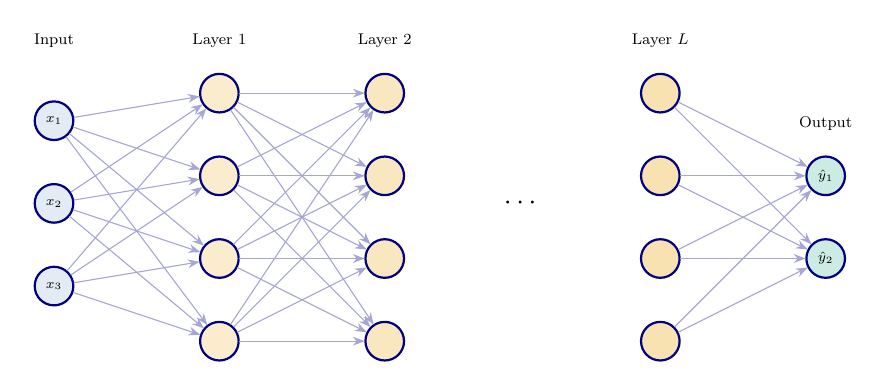
\begin{tikzpicture}[scale=0.7, transform shape,
    neuron/.style={circle, draw=uzhblue, thick, minimum size=7mm},
    arr/.style={-{Stealth[length=1.5mm]}, uzhblue!35}]

    % Input layer
    \foreach \i/\y in {1/2,2/0.5,3/-1} {
        \node[neuron, fill=softblue!15, font=\scriptsize] (x\i) at (0,\y) {$x_\i$};
    }
    % Hidden 1
    \foreach \i/\y in {1/2.5,2/1,3/-0.5,4/-2} {
        \node[neuron, fill=softorange!20, font=\tiny] (h1\i) at (3,\y) {};
    }
    % Hidden 2
    \foreach \i/\y in {1/2.5,2/1,3/-0.5,4/-2} {
        \node[neuron, fill=softorange!25, font=\tiny] (h2\i) at (6,\y) {};
    }
    % Hidden L
    \foreach \i/\y in {1/2.5,2/1,3/-0.5,4/-2} {
        \node[neuron, fill=softorange!30, font=\tiny] (hL\i) at (11,\y) {};
    }
    % Output
    \foreach \i/\y in {1/1,2/-0.5} {
        \node[neuron, fill=softgreen!20, font=\scriptsize] (y\i) at (14,\y) {$\hat{y}_\i$};
    }

    % Dots
    \node[font=\Large] at (8.5,0.5) {$\cdots$};

    % Connections
    \foreach \i in {1,2,3} { \foreach \j in {1,2,3,4} { \draw[arr] (x\i)--(h1\j); }}
    \foreach \i in {1,2,3,4} { \foreach \j in {1,2,3,4} { \draw[arr] (h1\i)--(h2\j); }}
    \foreach \i in {1,2,3,4} { \foreach \j in {1,2} { \draw[arr] (hL\i)--(y\j); }}

    % Layer labels
    \node[font=\footnotesize, above] at (0,3.2) {Input};
    \node[font=\footnotesize, above] at (3,3.2) {Layer 1};
    \node[font=\footnotesize, above] at (6,3.2) {Layer 2};
    \node[font=\footnotesize, above] at (11,3.2) {Layer $L$};
    \node[font=\footnotesize, above] at (14,1.7) {Output};
\end{tikzpicture}
\end{center}

\vspace{0.1cm}
An $L$-layer network computes a nested composition:
\[
    \boxed{f(\x;\bm{\theta}) = g_L\!\Big(\W^{(L)} g_{L-1}\!\big(\cdots g_1\!\big(\W^{(1)}\x + \bb^{(1)}\big)\cdots + \bb^{(L-1)}\big) + \bb^{(L)}\Big)}
\]

{\small Each layer transforms the representation.  \textbf{Depth} provides exponential gains in representational power over width alone.}
\end{frame}

% --- Slide 25: Universal Approximation ---
\begin{frame}{Universal Approximation Theorem}
\small
\begin{block}{Theorem (Cybenko 1989; Hornik, Stinchcombe \& White 1989)}
Let $g:\R\to\R$ be a bounded, non-constant, continuous activation function.  Then for any continuous function $f:\mathcal{K}\to\R$ on a compact set $\mathcal{K}\subset\R^d$ and any $\varepsilon>0$, there exists a single-hidden-layer network
\[
    F(\x) = \sum_{j=1}^{n_1} v_j\, g\!\big(\w_j^\top\x + b_j\big)
\]
such that $\sup_{\x\in\mathcal{K}} |F(\x) - f(\x)| < \varepsilon$.
\end{block}

\vspace{0.25cm}
\textbf{Caveats:}
\begin{itemize}\itemsep0pt
    \item The required width $n_1$ may be \textbf{exponentially large} in $d$.
    \item Existence $\neq$ efficient learnability.
    \item Practical success of deep learning suggests that \textbf{depth} provides a much more efficient parameterization than width alone.
\end{itemize}
\end{frame}

% --- Slide 26: Geometric View ---
\begin{frame}{A Geometric View: Learning to Untangle}
Neural networks learn \textbf{successive coordinate transformations} that make the data linearly separable.

\vspace{0.3cm}
\begin{center}
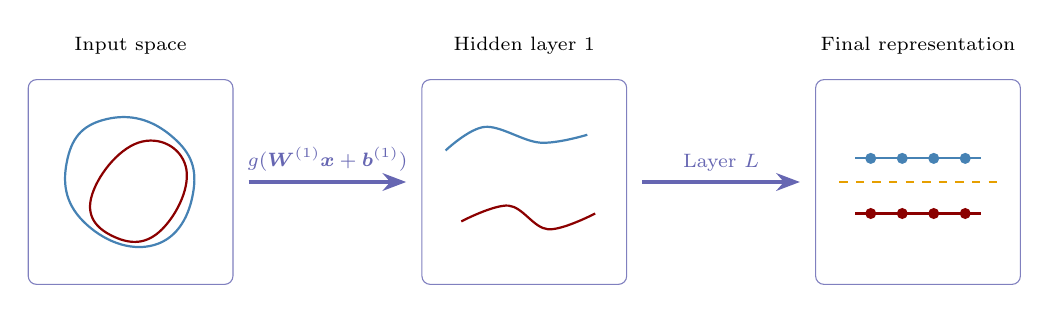
\begin{tikzpicture}[
    box/.style={rectangle, draw=uzhblue!50, rounded corners=3pt,
                minimum width=2.6cm, minimum height=2.6cm, inner sep=0pt},
    arr/.style={-{Stealth[length=3mm]}, very thick, uzhblue!60}
]
    % Panel 1: tangled
    \node[box] (p1) at (0,0) {};
    \node[font=\scriptsize, above] at (0,1.5) {Input space};
    % Draw tangled pattern
    \draw[softblue, thick] plot[smooth cycle, tension=0.8] coordinates {
        (-0.8,0.3) (-0.3,0.8) (0.5,0.6) (0.8,-0.1) (0.3,-0.8) (-0.6,-0.5)};
    \draw[darkred, thick] plot[smooth cycle, tension=0.8] coordinates {
        (-0.5,-0.2) (0.1,0.5) (0.7,0.2) (0.4,-0.6) (-0.2,-0.7)};

    % Arrow 1
    \draw[arr] (1.5,0) -- node[above, font=\scriptsize]{$g(\W^{(1)}\x+\bb^{(1)})$} (3.5,0);

    % Panel 2: partially untangled
    \node[box] (p2) at (5,0) {};
    \node[font=\scriptsize, above] at (5,1.5) {Hidden layer 1};
    \draw[softblue, thick] plot[smooth, tension=0.6] coordinates {
        (4.0,0.4) (4.5,0.7) (5.2,0.5) (5.8,0.6)};
    \draw[darkred, thick] plot[smooth, tension=0.6] coordinates {
        (4.2,-0.5) (4.8,-0.3) (5.3,-0.6) (5.9,-0.4)};

    % Arrow 2
    \draw[arr] (6.5,0) -- node[above, font=\scriptsize]{Layer $L$} (8.5,0);

    % Panel 3: linearly separable
    \node[box] (p3) at (10,0) {};
    \node[font=\scriptsize, above] at (10,1.5) {Final representation};
    % Separated
    \draw[softblue, thick] (9.2,0.3) -- (10.8,0.3);
    \fill[softblue] (9.4,0.3) circle (2pt);
    \fill[softblue] (9.8,0.3) circle (2pt);
    \fill[softblue] (10.2,0.3) circle (2pt);
    \fill[softblue] (10.6,0.3) circle (2pt);
    \draw[darkred, thick] (9.2,-0.4) -- (10.8,-0.4);
    \fill[darkred] (9.4,-0.4) circle (2pt);
    \fill[darkred] (9.8,-0.4) circle (2pt);
    \fill[darkred] (10.2,-0.4) circle (2pt);
    \fill[darkred] (10.6,-0.4) circle (2pt);
    % Separating line
    \draw[softorange, thick, dashed] (9.0,0) -- (11.0,0);
\end{tikzpicture}
\end{center}

\vspace{0.2cm}
{\small Analogy (Chollet, 2017): imagine crumpling two sheets of colored paper into a ball. A neural network learns how to smooth them out again, layer by layer, until a simple linear classifier can separate the colors.}
\end{frame}

% --- The Crumpling Analogy ---
\begin{frame}{The Paper-Crumpling Analogy (Chollet, 2017)}
\begin{columns}[c]
\column{0.55\textwidth}
\begin{center}
\includegraphics[width=\textwidth]{figures/crumple.png}
\end{center}

\column{0.42\textwidth}
Each layer of a deep network applies a simple geometric transformation:
\begin{itemize}
    \item \textbf{Affine map} $\W\x + \bb$ (rotation, scaling, translation)
    \item \textbf{Activation} $g(\cdot)$ (folding, warping)
\end{itemize}

\vspace{0.3cm}
Together, many layers ``uncrumple'' the data manifold until the classes become linearly separable.
\end{columns}
\end{frame}

% ============================================================================
% PART 4: TRAINING NEURAL NETWORKS
% ============================================================================

\section{Training Neural Networks}

% --- Section Divider ---
\begin{frame}{}
\begin{center}
{\Huge \textcolor{uzhblue}{Part III}}\\[0.8em]
{\LARGE Training: Loss, Gradients, and Optimization}
\end{center}
\end{frame}

% --- Slide 28: Loss Functions ---
\begin{frame}{Loss Functions}
The loss function $J(\bm{\theta})$ measures how far predictions $\hat{\bm{y}}$ are from targets $\bm{y}$.

\vspace{0.4cm}
\begin{columns}[T]
\column{0.48\textwidth}
\begin{block}{Regression: Mean Squared Error}
\[
    J(\bm{\theta}) = \frac{1}{m}\sum_{i=1}^{m}\big(y^{(i)} - f(\x^{(i)};\bm{\theta})\big)^{2}
\]
Penalizes large deviations quadratically.
\end{block}

\column{0.48\textwidth}
\begin{block}{Classification: Cross-Entropy}
{\small
\[
    J = -\frac{1}{n}\sum_{i=1}^{n}\!\Big[y^{(i)}\!\log\hat{y}^{(i)} + (1{-}y^{(i)})\log(1{-}\hat{y}^{(i)})\Big]
\]}%
\vspace{-0.3cm}

For binary labels $y\in\{0,1\}$.
\end{block}
\end{columns}

\vspace{0.3cm}
\textbf{Multiclass} ($K$ classes): use softmax output $\hat{y}_k = e^{z_k}\big/\sum_j e^{z_j}$ and categorical cross-entropy:
$J = -\frac{1}{n}\sum_{i}\sum_{k} y_k^{(i)}\log \hat{y}_k^{(i)}$.
\end{frame}

% --- Slide 28a: Beyond MSE ---
\begin{frame}[shrink=10]{Beyond MSE: Robust and Asymmetric Losses}
\begin{columns}[T]
\column{0.50\textwidth}
{\small
Let $r = y - \hat{y}$ denote the residual.

\vspace{0.1cm}
\textbf{MAE (L1):}\quad robust to outliers (constant gradient)
\vspace{-0.15cm}
\[
    L_{\text{MAE}} = \tfrac{1}{n}\textstyle\sum_{i=1}^{n}\big|r^{(i)}\big|
\]

\vspace{-0.25cm}
\textbf{Huber ($\delta$):}\quad smooth near zero, linear in the tails
\vspace{-0.15cm}
\[
    L_\delta(r) = \begin{cases} \tfrac{1}{2}r^2 & |r|\le\delta \\[2pt] \delta\!\left(|r|-\tfrac{\delta}{2}\right) & |r|>\delta\end{cases}
\]

\vspace{-0.25cm}
\textbf{Quantile / Pinball ($\tau\!\in\!(0,1)$):}
\vspace{-0.15cm}
\[
    L_\tau(r) = \begin{cases} \tau\,|r| & r \ge 0 \;\;(\text{under-predict})\\[2pt] (1{-}\tau)\,|r| & r < 0 \;\;(\text{over-predict})\end{cases}
\]

\vspace{-0.25cm}
$\tau{>}0.5$: penalises under-prediction more $\Rightarrow$ predicts \emph{high} quantile.
Directly gives VaR at level $\tau$.
}%

\column{0.46\textwidth}
\begin{center}
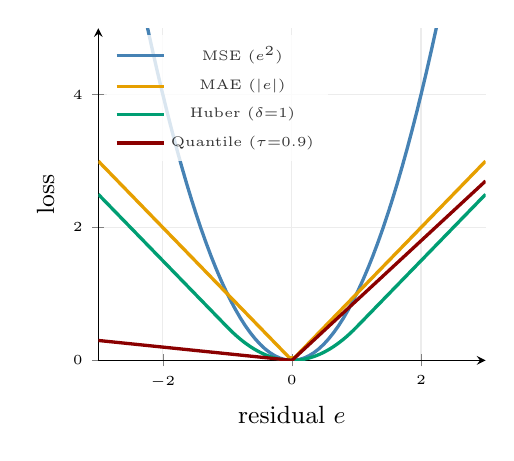
\begin{tikzpicture}
\begin{axis}[
    width=6.5cm, height=5.8cm,
    xlabel={residual $e$},
    ylabel={loss},
    xlabel style={font=\small},
    ylabel style={font=\small},
    tick label style={font=\tiny},
    xmin=-3, xmax=3, ymin=0, ymax=5,
    grid=major, grid style={gray!15},
    axis lines=left,
    legend style={font=\tiny, at={(0.02,0.98)}, anchor=north west,
                  row sep=1pt, draw=none, fill=white, fill opacity=0.8},
]
    % MSE: e^2
    \addplot[very thick, softblue, domain=-3:3, samples=80]{x^2};
    \addlegendentry{MSE ($e^2$)}
    % MAE: |e|
    \addplot[very thick, softorange, domain=-3:3, samples=80]{abs(x)};
    \addlegendentry{MAE ($|e|$)}
    % Huber (delta=1) — softgreen for high contrast against darkred Quantile
    \addplot[very thick, softgreen, domain=-3:-1, samples=40]{abs(x) - 0.5};
    \addplot[very thick, softgreen, forget plot, domain=-1:1, samples=40]{0.5*x^2};
    \addplot[very thick, softgreen, forget plot, domain=1:3, samples=40]{abs(x) - 0.5};
    \addlegendentry{Huber ($\delta{=}1$)}
    % Quantile (tau=0.9)
    \addplot[very thick, darkred, domain=-3:0, samples=40]{-0.1*x};
    \addplot[very thick, darkred, forget plot, domain=0:3, samples=40]{0.9*x};
    \addlegendentry{Quantile ($\tau{=}0.9$)}
\end{axis}
\end{tikzpicture}
\end{center}
\end{columns}
\end{frame}

% --- Slide 28b: Choosing a Loss Function ---
\begin{frame}[shrink=10]{Choosing a Loss Function}
\begin{center}
{\small
\renewcommand{\arraystretch}{1.4}
\begin{tabular}{lcccc}
\toprule
\textbf{Loss} & \textbf{Outliers} & \textbf{Smoothness} & \textbf{Symmetry} & \textbf{Use case} \\
\midrule
MSE      & High & Smooth          & Symmetric           & Default regression \\
MAE      & Low  & Non-smooth at 0 & Symmetric           & Median regression \\
Huber    & Low  & Smooth          & Symmetric           & Robust regression \\
Quantile & Low  & Non-smooth at 0 & \textbf{Asymmetric} & Risk, VaR, tails \\
\bottomrule
\end{tabular}
}%
\end{center}

\vspace{0.5cm}
\begin{alertblock}{Why this matters in economics and finance}
Tail risks are often more important than average performance.
\textbf{Quantile loss} lets the model focus on getting worst-case predictions right,
directly producing Value-at-Risk (VaR) or Expected Shortfall estimates.
See \textbf{Notebook~07} for a hands-on comparison.
\end{alertblock}

\vspace{0.2cm}
{\small \textbf{References:} Huber (1964), Koenker \& Bassett (1978).}
\end{frame}

% --- Slide 29: Gradient Descent Idea ---
\begin{frame}{Gradient Descent -- The Idea}
\begin{columns}[T]
\column{0.48\textwidth}
\textbf{Goal:} find weights that minimize the loss:
\[
    \bm{\theta}^{*} = \argmin_{\bm{\theta}}\; J(\bm{\theta})
\]

\textbf{Strategy:} start from a random point, repeatedly step in the direction of steepest descent:
\[
    \bm{\theta} \;\leftarrow\; \bm{\theta} - \eta\,\nabla_{\!\bm{\theta}} J(\bm{\theta})
\]

where $\eta > 0$ is the \textbf{learning rate}.

\column{0.48\textwidth}
\begin{center}
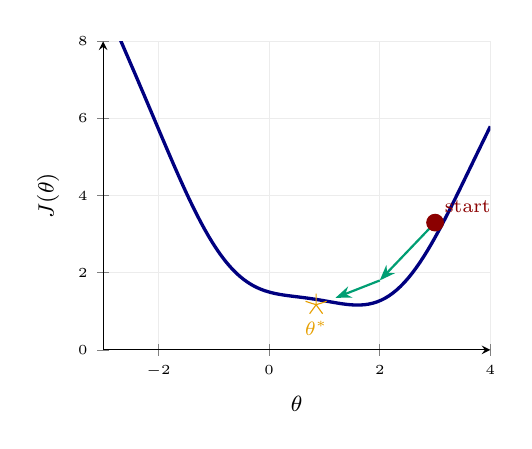
\begin{tikzpicture}
\begin{axis}[
    width=6.5cm, height=5.5cm,
    xlabel={$\theta$}, ylabel={$J(\theta)$},
    xlabel style={font=\footnotesize},
    ylabel style={font=\footnotesize},
    tick label style={font=\tiny},
    xmin=-3, xmax=4, ymin=0, ymax=8,
    grid=major, grid style={gray!15},
    axis lines=left,
    ytick={0,2,4,6,8},
]
    % Loss curve
    \addplot[very thick, uzhblue, domain=-3:4, samples=100]{0.5*(x-1)^2 + 0.3*sin(deg(x*2)) + 1};
    % Starting point
    \addplot[only marks, mark=*, mark size=3pt, darkred] coordinates {(3, 3.3)};
    \node[font=\scriptsize, darkred, above right] at (axis cs:3,3.3) {start};
    % Arrow showing descent
    \draw[-{Stealth[length=2mm]}, thick, softgreen] (axis cs:3,3.3) -- (axis cs:2,1.8);
    \draw[-{Stealth[length=2mm]}, thick, softgreen] (axis cs:2,1.8) -- (axis cs:1.2,1.35);
    % Minimum
    \addplot[only marks, mark=star, mark size=4pt, softorange] coordinates {(0.85, 1.17)};
    \node[font=\scriptsize, softorange, below] at (axis cs:0.85,1.0) {$\theta^*$};
\end{axis}
\end{tikzpicture}
\end{center}
\end{columns}
\end{frame}

% --- Slide 30: GD Algorithm ---
\begin{frame}{Gradient Descent Algorithm}
\begin{columns}[T]
\column{0.55\textwidth}
\begin{algorithm}[H]
\caption*{\textbf{Gradient Descent}}
\begin{algorithmic}[1]
\STATE Initialize $\bm{\theta} \sim \mathcal{N}(\bm{0}, \sigma^2\bm{I})$
\REPEAT
    \STATE Compute gradient: $\bm{g} \leftarrow \nabla_{\!\bm{\theta}} J(\bm{\theta})$
    \STATE Update weights: $\bm{\theta} \leftarrow \bm{\theta} - \eta\,\bm{g}$
\UNTIL{convergence}
\RETURN $\bm{\theta}$
\end{algorithmic}
\end{algorithm}

\column{0.42\textwidth}
\textbf{Key considerations:}
\begin{itemize}
    \item Computing $\nabla J$ over \emph{all} $n$ training points is $O(n)$ per step, expensive for large datasets.
    \item The learning rate $\eta$ controls step size.
    \item Convergence is to a \textbf{local} minimum (loss landscapes are non-convex for neural networks).
\end{itemize}
\end{columns}
\end{frame}

% --- Slide 31: SGD ---
\begin{frame}[shrink=8]{Stochastic Gradient Descent (SGD)}
\textbf{Idea:} approximate the full gradient with a cheap estimate from a small subset of data.

\vspace{0.3cm}
\begin{columns}[T]
\column{0.48\textwidth}
\begin{block}{Single-sample SGD}
Pick one random example $(\x^{(i)},y^{(i)})$:
\[
    \bm{\theta} \leftarrow \bm{\theta} - \eta\,\nabla_{\!\bm{\theta}} J_i(\bm{\theta})
\]
Cheap but noisy.
\end{block}

\column{0.48\textwidth}
\begin{block}{Mini-batch SGD}
Sample a batch $\mathcal{B}$ of $B$ examples:
\[
    \bm{\theta} \leftarrow \bm{\theta} - \frac{\eta}{B}\sum_{k\in\mathcal{B}} \nabla_{\!\bm{\theta}} J_k(\bm{\theta})
\]
Reduces variance; enables GPU parallelism.
\end{block}
\end{columns}

\vspace{0.15cm}
{\small\textbf{Why does this work?} The mini-batch gradient is an \textbf{unbiased estimate} of the full gradient:}
\vspace{-0.15cm}
\[
    \E{\frac{1}{B}\sum_{k\in\mathcal{B}}\nabla J_k} = \nabla J
\]
\vspace{-0.4cm}

{\small Unbiased estimates suffice for convergence (Robbins \& Monro, 1951).}
\end{frame}

% --- Slide 32: Mini-batches and Epochs ---
\begin{frame}{Mini-Batches and Epochs}
\begin{center}
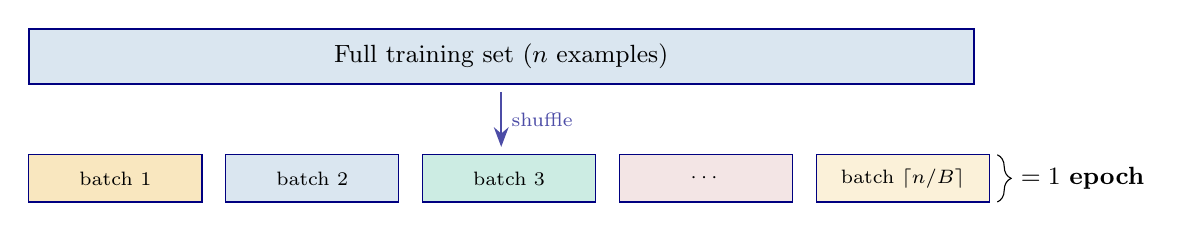
\begin{tikzpicture}[
    box/.style={rectangle, draw=uzhblue, rounded corners=3pt, minimum height=8mm, font=\small, inner sep=4pt},
    arr/.style={-{Stealth[length=2.5mm]}, thick, uzhblue!70}
]
    % Training data bar
    \fill[softblue!20] (0,0) rectangle (12,0.7);
    \draw[uzhblue, thick] (0,0) rectangle (12,0.7);
    \node[font=\small] at (6, 0.35) {Full training set ($n$ examples)};

    % Shuffle arrow
    \draw[arr] (6,-0.1) -- (6,-0.8) node[right, font=\scriptsize, pos=0.5]{shuffle};

    % Mini-batches
    \foreach \i/\c in {0/softorange!25, 2.5/softblue!20, 5/softgreen!20, 7.5/darkred!10, 10/softorange!15} {
        \fill[\c] (\i,-1.5) rectangle (\i+2.2,-0.9);
        \draw[uzhblue] (\i,-1.5) rectangle (\i+2.2,-0.9);
    }
    \node[font=\scriptsize] at (1.1,-1.2) {batch 1};
    \node[font=\scriptsize] at (3.6,-1.2) {batch 2};
    \node[font=\scriptsize] at (6.1,-1.2) {batch 3};
    \node[font=\scriptsize] at (8.6,-1.2) {$\cdots$};
    \node[font=\scriptsize] at (11.1,-1.2) {batch $\lceil n/B\rceil$};

    % Brace for epoch
    \draw[decorate, decoration={brace, amplitude=5pt}] (12.3,-0.9) -- (12.3,-1.5)
        node[midway, right=5pt, font=\small]{$= 1$ \textbf{epoch}};
\end{tikzpicture}
\end{center}

\vspace{0.5cm}
\begin{itemize}
    \item One \textbf{epoch} = one complete pass through the training set.
    \item Typical batch sizes: $B \in \{32, 64, 128, 256\}$.
    \item Benefits of mini-batches:
    \begin{itemize}
        \item[\textendash] Smoother convergence than single-sample SGD.
        \item[\textendash] Efficient use of GPU parallelism.
        \item[\textendash] Implicit regularization from gradient noise.
    \end{itemize}
\end{itemize}
\end{frame}

% --- Slide 33: Backpropagation Key Idea ---
\begin{frame}{Backpropagation -- The Key Idea}
\textbf{Problem:} how do we compute $\frac{\partial J}{\partial \W^{(\ell)}}$ for each layer $\ell$?

\vspace{0.3cm}
\textbf{Answer:} the \textbf{chain rule} of calculus, applied systematically.

\vspace{0.4cm}
\begin{center}
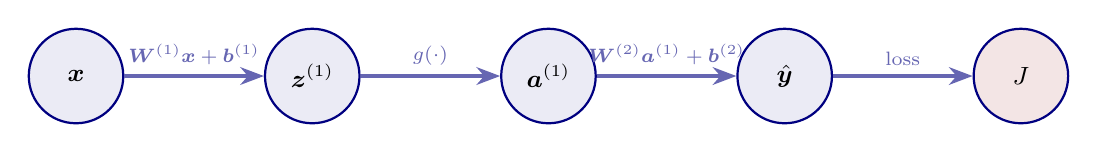
\begin{tikzpicture}[
    node/.style={circle, draw=uzhblue, thick, minimum size=12mm, fill=uzhblue!8, font=\small},
    arr/.style={-{Stealth[length=3mm]}, very thick, uzhblue!60}
]
    \node[node] (x) at (0,0) {$\x$};
    \node[node] (z1) at (3,0) {$\z^{(1)}$};
    \node[node] (a1) at (6,0) {$\a^{(1)}$};
    \node[node] (yhat) at (9,0) {$\hat{\bm{y}}$};
    \node[node, fill=darkred!10] (J) at (12,0) {$J$};

    \draw[arr] (x) -- node[above, font=\scriptsize]{$\W^{(1)}\x+\bb^{(1)}$} (z1);
    \draw[arr] (z1) -- node[above, font=\scriptsize]{$g(\cdot)$} (a1);
    \draw[arr] (a1) -- node[above, font=\scriptsize]{$\W^{(2)}\a^{(1)}+\bb^{(2)}$} (yhat);
    \draw[arr] (yhat) -- node[above, font=\scriptsize]{loss} (J);
\end{tikzpicture}
\end{center}

\vspace{0.3cm}
\[
    \frac{\partial J}{\partial \W^{(1)}} = \underbrace{\frac{\partial J}{\partial \hat{\bm{y}}}}_{\text{output error}} \cdot \underbrace{\frac{\partial \hat{\bm{y}}}{\partial \a^{(1)}}}_{\W^{(2)}} \cdot \underbrace{\frac{\partial \a^{(1)}}{\partial \z^{(1)}}}_{g'(\z^{(1)})} \cdot \underbrace{\frac{\partial \z^{(1)}}{\partial \W^{(1)}}}_{\x}
\]
\end{frame}

% --- Slide 34: Backpropagation Forward Pass ---
\begin{frame}{Backpropagation -- Forward Pass}
Given input $\x$, compute layer by layer and \textbf{store all intermediate quantities}:

\vspace{0.3cm}
\begin{center}
\renewcommand{\arraystretch}{1.4}
\begin{tabular}{rll}
\toprule
\textbf{Layer} & \textbf{Pre-activation} & \textbf{Activation} \\
\midrule
$\ell = 0$ & & $\a^{(0)} = \x$ \\
$\ell = 1$ & $\z^{(1)} = \W^{(1)}\a^{(0)} + \bb^{(1)}$ & $\a^{(1)} = g(\z^{(1)})$ \\
$\ell = 2$ & $\z^{(2)} = \W^{(2)}\a^{(1)} + \bb^{(2)}$ & $\a^{(2)} = g(\z^{(2)})$ \\
$\vdots$ & $\vdots$ & $\vdots$ \\
$\ell = L$ & $\z^{(L)} = \W^{(L)}\a^{(L-1)} + \bb^{(L)}$ & $\hat{\bm{y}} = g_{\text{out}}(\z^{(L)})$ \\
\bottomrule
\end{tabular}
\end{center}

\vspace{0.2cm}
Finally compute the loss: $J = \ell\big(\bm{y},\, \hat{\bm{y}}\big)$.
We need all the $\z^{(\ell)}$ and $\a^{(\ell)}$ values for the backward pass.
\end{frame}

% --- Slide 35: Backpropagation Backward Pass ---
\begin{frame}{Backpropagation -- Backward Pass}
Define the \textbf{error signal} at layer $\ell$:
\[
    \bm{\delta}^{(\ell)} \;\equiv\; \frac{\partial J}{\partial \z^{(\ell)}} \;\in\;\R^{n_\ell}
\]

\vspace{0.2cm}
\textbf{Output layer} ($\ell = L$):
\[
    \bm{\delta}^{(L)} = \nabla_{\!\z^{(L)}} J = \frac{\partial J}{\partial \hat{\bm{y}}}\odot g_{\text{out}}'(\z^{(L)})
\]

\textbf{Hidden layers} ($\ell = L{-}1, \dots, 1$)~~---~~propagate error \textit{backward}:
\[
    \boxed{\bm{\delta}^{(\ell)} = \big(\W^{(\ell+1)}\big)^{\!\top}\bm{\delta}^{(\ell+1)} \;\odot\; g'\!\big(\z^{(\ell)}\big)}
\]

\textbf{Parameter gradients:}
\[
    \frac{\partial J}{\partial \W^{(\ell)}} = \bm{\delta}^{(\ell)}\big(\a^{(\ell-1)}\big)^{\!\top}, \qquad
    \frac{\partial J}{\partial \bb^{(\ell)}} = \bm{\delta}^{(\ell)}
\]

{\small The symbol $\odot$ denotes the element-wise (Hadamard) product.}
\end{frame}

% --- Slide 36: Learning Rate ---
\begin{frame}{The Learning Rate}
\begin{center}
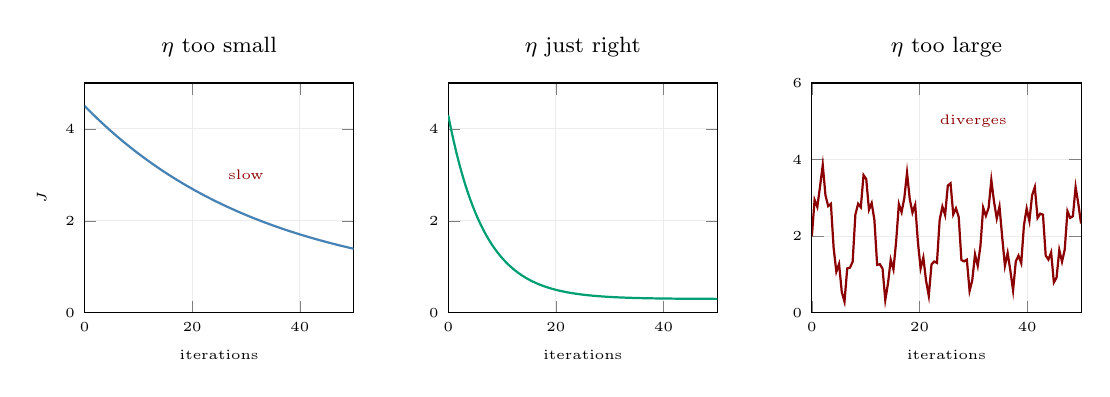
\begin{tikzpicture}
\begin{axis}[
    name=plotL,
    width=5cm, height=4.5cm,
    title={\footnotesize $\eta$ too small},
    title style={font=\footnotesize},
    xlabel={iterations}, ylabel={$J$},
    xlabel style={font=\tiny}, ylabel style={font=\tiny},
    tick label style={font=\tiny},
    xmin=0, xmax=50, ymin=0, ymax=5,
    grid=major, grid style={gray!15},
]
    \addplot[thick, softblue, domain=0:50, samples=100]{4*exp(-0.03*x)+0.5};
    \node[font=\tiny, darkred] at (axis cs:30,3) {slow};
\end{axis}

\begin{axis}[
    at={($(plotL.east)+(1.2cm,0)$)}, anchor=west,
    name=plotM,
    width=5cm, height=4.5cm,
    title={\footnotesize $\eta$ just right},
    title style={font=\footnotesize},
    xlabel={iterations},
    xlabel style={font=\tiny},
    tick label style={font=\tiny},
    xmin=0, xmax=50, ymin=0, ymax=5,
    grid=major, grid style={gray!15},
]
    \addplot[thick, softgreen, domain=0:50, samples=100]{4*exp(-0.15*x)+0.3};
\end{axis}

\begin{axis}[
    at={($(plotM.east)+(1.2cm,0)$)}, anchor=west,
    width=5cm, height=4.5cm,
    title={\footnotesize $\eta$ too large},
    title style={font=\footnotesize},
    xlabel={iterations},
    xlabel style={font=\tiny},
    tick label style={font=\tiny},
    xmin=0, xmax=50, ymin=0, ymax=6,
    grid=major, grid style={gray!15},
]
    \addplot[thick, darkred, domain=0:50, samples=100]{2+1.5*sin(deg(x*0.8))*exp(-0.01*x)+0.4*sin(deg(x*4))};
    \node[font=\tiny, darkred] at (axis cs:30,5) {diverges};
\end{axis}
\end{tikzpicture}
\end{center}

\vspace{0.3cm}
\begin{itemize}
    \item \textbf{Too small:} slow convergence, may get stuck in poor local minima.
    \item \textbf{Too large:} oscillation or divergence, overshooting the minimum.
    \item \textbf{Solution:} use \textbf{adaptive learning rates} that adjust automatically.
\end{itemize}
\end{frame}

% --- Intermezzo: Hands-on (GD / SGD / learning rate) ---
\begin{frame}{Intermezzo -- Hands-On}
\begin{block}{Gradient Descent Notebook}
Open and work through: \textbf{lectures/lecture\_02\_intro\_deep\_learning/code/lecture\_02\_02\_GradientDescent\_and\_StochasticGradientDescent.ipynb}
\end{block}

\vspace{0.5cm}
\textbf{In this notebook, you will:}
\begin{enumerate}
    \item Implement gradient descent from scratch for a simple function.
    \item Compare full-batch GD with stochastic (per-sample) SGD.
    \item Visualize how the learning rate affects convergence.
\end{enumerate}

\vspace{0.5cm}
\begin{center}
{\small Log in and launch the ``Deep Learning for Econ'' application.}
\end{center}
\end{frame}

% --- Slide 37: Adaptive Optimizers ---
\begin{frame}{Adaptive Optimizers}
\begin{small}
\renewcommand{\arraystretch}{1.25}
\begin{tabular}{lp{9cm}}
\toprule
\textbf{Method} & \textbf{Update rule} \\
\midrule
\textbf{Momentum} & $\bm{v}_t = \mu\,\bm{v}_{t-1} + \nabla J(\bm{\theta}_t)$;~~$\bm{\theta}_{t+1} = \bm{\theta}_t - \eta\,\bm{v}_t$ \\[2pt]
\textbf{RMSProp} & $\bm{s}_t = \beta\,\bm{s}_{t-1} + (1-\beta)(\nabla J)^2$;~~$\bm{\theta}_{t+1} = \bm{\theta}_t - \frac{\eta}{\sqrt{\bm{s}_t + \varepsilon}}\odot\nabla J$ \\[2pt]
\textbf{Adam} & $\bm{m}_t = \beta_1\bm{m}_{t-1} + (1-\beta_1)\nabla J$~~~~(1st moment) \\
& $\bm{v}_t = \beta_2\bm{v}_{t-1} + (1-\beta_2)(\nabla J)^2$~~~~(2nd moment) \\
& $\hat{\bm{m}}_t = \bm{m}_t/(1-\beta_1^t)$,~~$\hat{\bm{v}}_t = \bm{v}_t/(1-\beta_2^t)$~~~~(bias correction) \\
& $\bm{\theta}_{t+1} = \bm{\theta}_t - \eta\,\hat{\bm{m}}_t \big/ (\sqrt{\hat{\bm{v}}_t} + \varepsilon)$ \\[2pt]
\textbf{AdamW} & $\bm{\theta}_{t+1} = (1-\eta\lambda)\bm{\theta}_t - \eta\,\hat{\bm{m}}_t \big/ (\sqrt{\hat{\bm{v}}_t} + \varepsilon)$~~~~(decoupled weight decay) \\
\bottomrule
\end{tabular}
\end{small}

\vspace{0.2cm}
{\footnotesize \textbf{Adam} (Kingma \& Ba, 2015) is the usual default ($\beta_1=0.9$, $\beta_2=0.999$, $\varepsilon=10^{-8}$).  \textbf{AdamW} (Loshchilov \& Hutter, 2019) decouples weight decay from the adaptive update, and is our default for PINN training in later chapters.}
\end{frame}

% --- Slide 38: Weight Initialization ---
\begin{frame}{Weight Initialization}
\textbf{Why not initialize all weights to zero?}
All neurons would compute the same output $\Rightarrow$ same gradient $\Rightarrow$ symmetry is never broken.

\vspace{0.12cm}
\textbf{Random initialization:} draw weights from a distribution scaled to the layer width $n_\ell$ (the number of neurons in layer~$\ell$; $n_{\ell-1}$ is then the fan-in from the previous layer).

\vspace{0.12cm}
\begin{columns}[T]
\column{0.48\textwidth}
\begin{block}{Xavier / Glorot (2010)}
For sigmoid or tanh activations:
\[
    W_{ij}^{(\ell)} \sim \mathcal{N}\!\left(0,\; \frac{2}{n_{\ell-1} + n_{\ell}}\right)
\]
Keeps activation variance roughly constant across layers.
\end{block}

\column{0.48\textwidth}
\begin{block}{He (2015)}
For ReLU activations:
\[
    W_{ij}^{(\ell)} \sim \mathcal{N}\!\left(0,\; \frac{2}{n_{\ell-1}}\right)
\]
Accounts for ReLU zeroing roughly half the variance.
\end{block}
\end{columns}

\vspace{0.1cm}
{\footnotesize Biases are typically initialized to zero. Proper initialization is critical for training deep networks.}
\end{frame}

% --- Slide 39: Vanishing and Exploding Gradients ---
\begin{frame}{Vanishing and Exploding Gradients}
\begin{columns}[T]
\column{0.52\textwidth}
The backward pass multiplies through many layers:
\[
    \bm{\delta}^{(\ell)} = \big(\W^{(\ell+1)}\big)^{\!\top}\bm{\delta}^{(\ell+1)}\odot g'(\z^{(\ell)})
\]

\begin{itemize}
    \item $|g'(z)| < 1$ at every layer $\Rightarrow$ product shrinks exponentially: \textbf{vanishing gradients}
    \item $|g'(z)| > 1$ or $\|\W^{(\ell)}\|$ large $\Rightarrow$ \textbf{exploding gradients}
\end{itemize}

\vspace{0.2cm}
\textbf{Remedies:} ReLU ($g'\in\{0,1\}$), proper initialization (He/Xavier), batch normalization, gradient clipping.

\column{0.45\textwidth}
\begin{center}
{\small\textbf{Sigmoid saturation zones}}
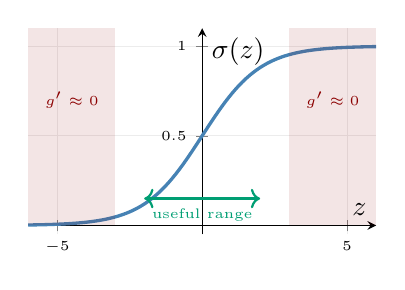
\begin{tikzpicture}
\begin{axis}[
    width=6cm, height=4.2cm,
    xlabel={$z$}, ylabel={$\sigma(z)$},
    xlabel style={font=\footnotesize},
    ylabel style={font=\footnotesize},
    tick label style={font=\tiny},
    xmin=-6, xmax=6, ymin=-0.05, ymax=1.1,
    grid=major, grid style={gray!15},
    axis lines=middle,
]
    \addplot[very thick, softblue, domain=-6:6, samples=100]{1/(1+exp(-x))};
    % Saturation zones
    \fill[darkred, opacity=0.1] (axis cs:-6,0) rectangle (axis cs:-3,1.1);
    \fill[darkred, opacity=0.1] (axis cs:3,0) rectangle (axis cs:6,1.1);
    \node[font=\tiny, darkred] at (axis cs:-4.5,0.7) {$g' \approx 0$};
    \node[font=\tiny, darkred] at (axis cs:4.5,0.7) {$g' \approx 0$};
    \draw[<->, thick, softgreen] (axis cs:-2,0.15) -- (axis cs:2,0.15)
        node[midway, below, font=\tiny]{useful range};
\end{axis}
\end{tikzpicture}
\end{center}
\end{columns}
\end{frame}

% --- Batch Normalization (a mitigation for vanishing/exploding activations) ---
\begin{frame}{Batch Normalization}
\textbf{Idea} (Ioffe \& Szegedy, 2015): normalize activations within each mini-batch to stabilize training.

\vspace{0.2cm}
For a mini-batch $\mathcal{B} = \{z_1, \dots, z_B\}$ at some layer:
\begin{align*}
    \mu_{\mathcal{B}} = \frac{1}{B}\sum_{i=1}^{B} z_i, \quad
    \sigma_{\mathcal{B}}^2 = \frac{1}{B}\sum_{i=1}^{B} (z_i - \mu_{\mathcal{B}})^2, \quad
    \hat{z}_i = \frac{z_i - \mu_{\mathcal{B}}}{\sqrt{\sigma_{\mathcal{B}}^2 + \varepsilon}}, \quad
    y_i = \gamma\, \hat{z}_i + \beta
\end{align*}

where $\gamma$ and $\beta$ are \textbf{learnable} scale and shift parameters.

\vspace{0.2cm}
\textbf{Benefits:}
\begin{itemize}
    \item Stabilizes training, allows higher learning rates.
    \item Mitigates vanishing/exploding activations across layers.
    \item Applied per-layer, typically before the activation function.
\end{itemize}

\vspace{0.1cm}
{\scriptsize \emphc{Variants beyond batch.}  LayerNorm, GroupNorm, and WeightNorm address the small-batch and recurrent settings; the script (\S\,Normalization Variants) treats them in detail.}
\end{frame}

% --- Batch Normalization: Intuition ---
\begin{frame}{Batch Normalization: Intuition}
\begin{columns}[T]
\column{0.52\textwidth}
\textbf{Why does BN help?}
\begin{itemize}\itemsep3pt
    \item[\textcolor{harvardcrimson}{$\blacktriangleright$}] {\small \emphc{The problem.} As earlier layers update, layer~$\ell$'s input distribution \emph{drifts} every step. Each layer chases a \textit{moving target} $\Rightarrow$ unstable gradients (\textit{internal covariate shift}).}
    \item[\textcolor{harvardcrimson}{$\blacktriangleright$}] {\small \emphc{The fix.} BN = standardize pre-activations every mini-batch (just like standardizing regressors). Each layer always sees inputs at $\mu{=}0,\sigma{=}1$ $\Rightarrow$ gradients flow predictably, larger learning rates become safe.}
    \item[\textcolor{harvardcrimson}{$\blacktriangleright$}] {\small \emphc{Why $\gamma,\beta$?} They are learnable: a layer that prefers non-standard inputs can shift them back. BN never reduces capacity, it just gives optimization a better starting point.}
\end{itemize}

\column{0.46\textwidth}
\begin{center}
{\small\textbf{Pre-activations $z$ at one hidden layer}}\\[0.16cm]

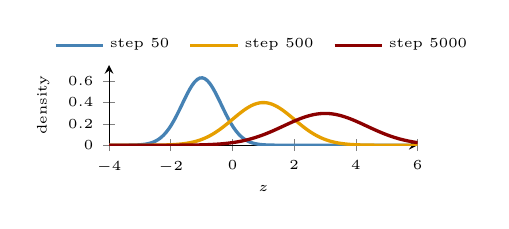
\begin{tikzpicture}
\begin{axis}[
    width=5.5cm, height=2.6cm,
    xmin=-4, xmax=6, ymin=0, ymax=0.75,
    xtick={-4,-2,0,2,4,6},
    xlabel={$z$}, xlabel style={font=\tiny, yshift=2pt},
    ylabel={density}, ylabel style={font=\tiny},
    tick label style={font=\tiny},
    axis lines=left, samples=120, no markers,
    legend style={font=\tiny, draw=none, fill=none,
                  at={(0.5,1.02)}, anchor=south, legend columns=-1,
                  /tikz/every even column/.append style={column sep=5pt}}
]
    \addplot[very thick, softblue,   domain=-4:6] {1/sqrt(2*pi*0.4)*exp(-(x+1)^2/(2*0.4))};
    \addlegendentry{step 50}
    \addplot[very thick, softorange, domain=-4:6] {1/sqrt(2*pi*1.0)*exp(-(x-1)^2/(2*1.0))};
    \addlegendentry{step 500}
    \addplot[very thick, darkred,    domain=-4:6] {1/sqrt(2*pi*1.8)*exp(-(x-3)^2/(2*1.8))};
    \addlegendentry{step 5000}
\end{axis}
\end{tikzpicture}\\[-0.1cm]
{\scriptsize\itshape Without BN: distribution drifts $\to$ moving target.}

\vspace{0.2cm}
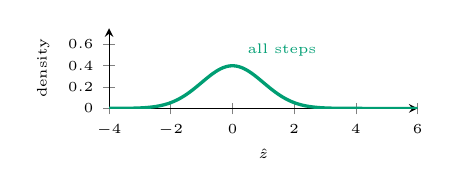
\begin{tikzpicture}
\begin{axis}[
    width=5.5cm, height=2.6cm,
    xmin=-4, xmax=6, ymin=0, ymax=0.75,
    xtick={-4,-2,0,2,4,6},
    xlabel={$\hat z$}, xlabel style={font=\tiny, yshift=2pt},
    ylabel={density}, ylabel style={font=\tiny},
    tick label style={font=\tiny},
    axis lines=left, samples=120, no markers,
]
    \addplot[very thick, softgreen, domain=-4:6] {1/sqrt(2*pi)*exp(-x^2/2)};
    \node[font=\tiny, softgreen] at (axis cs:1.6,0.55) {all steps};
\end{axis}
\end{tikzpicture}\\[-0.1cm]
{\scriptsize\itshape With BN: pinned to $\mathcal{N}(0,1)$ at every step.}
\end{center}
\end{columns}
\end{frame}

% --- Loss Landscape ---
\begin{frame}{Loss Landscapes of Neural Networks}
\begin{columns}[T]
\column{0.55\textwidth}
\begin{center}
\includegraphics[width=\textwidth]{figures/landscape.png}
\end{center}

\column{0.42\textwidth}
The loss surface of a deep network is highly non-convex:
\begin{itemize}
    \item Many \textbf{local minima} and \textbf{saddle points}
    \item Sharp vs.\ flat minima affect generalization
    \item SGD noise helps escape sharp minima
\end{itemize}

\vspace{0.3cm}
{\small Li et al.\ (2018): ``Visualizing the Loss Landscape of Neural Nets.''  Flat minima tend to generalize better than sharp ones.}
\end{columns}
\end{frame}

% --- Slide 40: Modern Activation Functions ---
\begin{frame}[shrink=10]{Modern Activation Functions: When to Use What}
{\footnotesize The common thread is \emphc{smoothness}. ReLU's kink at $z{=}0$ causes \textit{dead neurons} and an \textit{undefined second derivative}. Two families fix this; they differ only in whether they keep ReLU's asymptotic shape.}

\begin{columns}[T]
\column{0.55\textwidth}
\textbf{\textcolor{softblue}{Smooth \& ReLU-shaped}} {\footnotesize --- default for feedforward / CNN / attention:}
\begin{itemize}\itemsep0pt
    \item[\textcolor{softblue}{$\blacktriangleright$}] {\footnotesize \textbf{Swish/SiLU} $z\,\sigma(z)$: drop-in ReLU replacement (Ramachandran et al., 2017).}
    \item[\textcolor{harvardcrimson}{$\blacktriangleright$}] {\footnotesize \textbf{GELU} $z\,\Phi(z)$: transformer default (BERT, GPT, ViT).}
    \item[\textcolor{softgreen}{$\blacktriangleright$}] {\footnotesize \textbf{Mish} $z\tanh(\ln(1{+}e^z))$: modern vision (YOLOv4).}
\end{itemize}

\vspace{0.1cm}
\textbf{\textcolor{softorange}{Smooth, different shape}} {\footnotesize --- specialized outputs or differentiable losses:}
\begin{itemize}\itemsep0pt
    \item[\textcolor{softorange}{$\blacktriangleright$}] {\footnotesize \textbf{Softplus} $\ln(1{+}e^z)$: strictly positive $\Rightarrow$ variance heads ($\sigma^2$), Poisson rates.}
    \item[\textcolor{uzhblue}{$\blacktriangleright$}] {\footnotesize \textbf{tanh}: bounded $C^\infty$ $\Rightarrow$ PINNs (Day~6) where 2nd derivatives of the network enter the loss.}
\end{itemize}

\column{0.43\textwidth}
\begin{center}
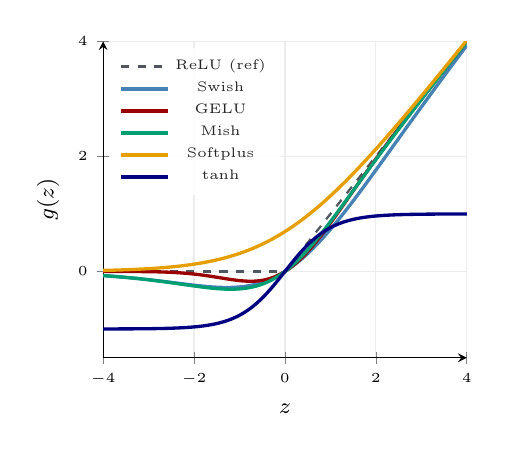
\begin{tikzpicture}
\begin{axis}[
    width=6.2cm, height=5.6cm,
    xlabel={$z$}, ylabel={$g(z)$},
    xlabel style={font=\footnotesize},
    ylabel style={font=\footnotesize},
    tick label style={font=\tiny},
    xmin=-4, xmax=4, ymin=-1.5, ymax=4,
    grid=major, grid style={gray!15},
    axis lines=left, samples=150, no markers,
    legend style={font=\tiny, draw=none, fill=white, fill opacity=0.85,
                  at={(0.02,0.98)}, anchor=north west, row sep=-1pt},
]
    % ReLU (baseline, gray dashed)
    \addplot[thick, uzhgreydark, dashed, domain=-4:0, samples=2]{0};
    \addlegendentry{ReLU (ref)}
    \addplot[thick, uzhgreydark, dashed, forget plot, domain=0:4, samples=2]{x};
    % Swish
    \addplot[very thick, softblue, domain=-4:4]{x/(1+exp(-x))};
    \addlegendentry{Swish}
    % GELU (tanh approximation)
    \addplot[very thick, harvardcrimson, domain=-4:4]
        {0.5*x*(1+tanh(0.7978845608*(x+0.044715*x*x*x)))};
    \addlegendentry{GELU}
    % Mish
    \addplot[very thick, softgreen, domain=-4:4]{x*tanh(ln(1+exp(x)))};
    \addlegendentry{Mish}
    % Softplus
    \addplot[very thick, softorange, domain=-4:4]{ln(1+exp(x))};
    \addlegendentry{Softplus}
    % tanh
    \addplot[very thick, uzhblue, domain=-4:4]{tanh(x)};
    \addlegendentry{tanh}
\end{axis}
\end{tikzpicture}
\end{center}
\end{columns}
\end{frame}

% ============================================================================
% PART 5: GENERALIZATION AND REGULARIZATION
% ============================================================================

\section{Generalization and Regularization}

% --- Section Divider ---
\begin{frame}{}
\begin{center}
{\Huge \textcolor{uzhblue}{Part IV}}\\[0.8em]
{\LARGE Generalization and Regularization}
\end{center}
\end{frame}

% --- Slide 42: Overfitting ---
\begin{frame}{Overfitting and Underfitting}
\begin{center}
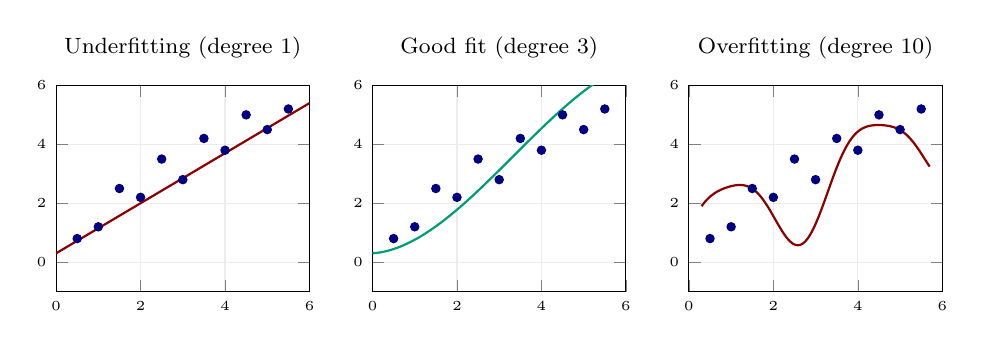
\begin{tikzpicture}
% Panel 1: Underfitting
\begin{axis}[
    name=p1,
    width=4.8cm, height=4.2cm,
    title={\footnotesize Underfitting (degree 1)},
    title style={font=\footnotesize},
    tick label style={font=\tiny},
    xmin=0, xmax=6, ymin=-1, ymax=6,
    grid=major, grid style={gray!15},
]
    \addplot[only marks, mark=*, mark size=1.5pt, uzhblue] coordinates {
        (0.5,0.8) (1,1.2) (1.5,2.5) (2,2.2) (2.5,3.5) (3,2.8) (3.5,4.2) (4,3.8) (4.5,5) (5,4.5) (5.5,5.2)
    };
    \addplot[thick, darkred, domain=0:6, samples=2]{0.3+0.85*x};
\end{axis}

% Panel 2: Good fit
\begin{axis}[
    at={($(p1.east)+(0.8cm,0)$)}, anchor=west,
    name=p2,
    width=4.8cm, height=4.2cm,
    title={\footnotesize Good fit (degree 3)},
    title style={font=\footnotesize},
    tick label style={font=\tiny},
    xmin=0, xmax=6, ymin=-1, ymax=6,
    grid=major, grid style={gray!15},
]
    \addplot[only marks, mark=*, mark size=1.5pt, uzhblue] coordinates {
        (0.5,0.8) (1,1.2) (1.5,2.5) (2,2.2) (2.5,3.5) (3,2.8) (3.5,4.2) (4,3.8) (4.5,5) (5,4.5) (5.5,5.2)
    };
    \addplot[thick, softgreen, domain=0:6, samples=100]{0.3+0.1*x+0.4*x^2-0.04*x^3};
\end{axis}

% Panel 3: Overfitting
\begin{axis}[
    at={($(p2.east)+(0.8cm,0)$)}, anchor=west,
    width=4.8cm, height=4.2cm,
    title={\footnotesize Overfitting (degree 10)},
    title style={font=\footnotesize},
    tick label style={font=\tiny},
    xmin=0, xmax=6, ymin=-1, ymax=6,
    grid=major, grid style={gray!15},
]
    \addplot[only marks, mark=*, mark size=1.5pt, uzhblue] coordinates {
        (0.5,0.8) (1,1.2) (1.5,2.5) (2,2.2) (2.5,3.5) (3,2.8) (3.5,4.2) (4,3.8) (4.5,5) (5,4.5) (5.5,5.2)
    };
    \addplot[thick, darkred, domain=0.3:5.7, samples=200]{
        0.8 + 1.5*sin(deg(x*1.8)) + 0.3*cos(deg(x*3.5)) + 0.6*x
    };
\end{axis}
\end{tikzpicture}
\end{center}

\vspace{0.2cm}
\begin{itemize}
    \item \textbf{Underfitting:} model too simple, high bias, cannot capture the pattern.
    \item \textbf{Overfitting:} model too complex, fits noise, poor generalization to new data.
    \item \textbf{Goal:} find the right complexity that generalizes well.
\end{itemize}
\end{frame}

% --- Slide 43: Train/Val/Test ---
\begin{frame}{Train / Validation / Test Split}
\begin{center}
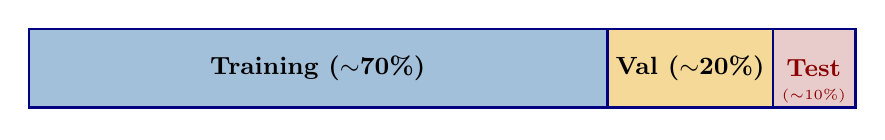
\begin{tikzpicture}
    % Full bar
    \fill[softblue!30] (0,0) rectangle (10.5,1);
    % Train
    \fill[softblue!50] (0,0) rectangle (7.35,1);
    % Val
    \fill[softorange!40] (7.35,0) rectangle (9.45,1);
    % Test
    \fill[darkred!20] (9.45,0) rectangle (10.5,1);
    % Borders
    \draw[uzhblue, thick] (0,0) rectangle (10.5,1);
    \draw[uzhblue, thick] (7.35,0) -- (7.35,1);
    \draw[uzhblue, thick] (9.45,0) -- (9.45,1);
    % Labels
    \node[font=\small\bfseries] at (3.67,0.5) {Training ($\sim$70\%)};
    \node[font=\small\bfseries] at (8.4,0.5) {Val ($\sim$20\%)};
    \node[font=\small\bfseries, darkred] at (9.97,0.5) {Test};
    \node[font=\tiny, darkred] at (9.97,0.15) {($\sim$10\%)};
\end{tikzpicture}
\end{center}

\vspace{0.4cm}
\begin{columns}[T]
\column{0.32\textwidth}
\begin{block}{\centering Training set}
    \centering
    {\small Used to fit model parameters $\bm{\theta}$ via optimization.}
\end{block}

\column{0.32\textwidth}
\begin{block}{\centering Validation set}
    \centering
    {\small Used for model selection: hyperparameters, architecture, early stopping.}
\end{block}

\column{0.32\textwidth}
\begin{block}{\centering Test set}
    \centering
    {\small Touched \textbf{once} at the very end to report final performance.}
\end{block}
\end{columns}

\vspace{0.3cm}
\begin{alertblock}{}
\centering Never use the test set for any decision during model development!
\end{alertblock}
\end{frame}

% --- Regularization Overview (concept map) ---
\begin{frame}{Regularization Techniques --- Overview}
\small
Goal: bias the learner toward \emphc{simpler} hypotheses so it generalizes beyond the training sample.

\vspace{0.3cm}
\begin{center}
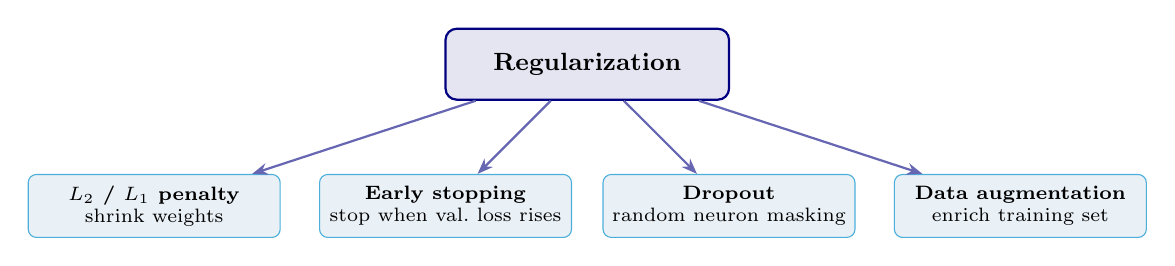
\begin{tikzpicture}[
    root/.style={rectangle, draw=uzhblue, thick, rounded corners=4pt,
                 fill=uzhblue!10, font=\small\bfseries,
                 minimum width=3.6cm, minimum height=0.9cm, align=center},
    leaf/.style={rectangle, draw=unil@blue!70, fill=softblue!12, rounded corners=3pt,
                 font=\scriptsize, minimum width=3.2cm, minimum height=0.8cm,
                 align=center, inner sep=3pt},
    arr/.style={-{Stealth[length=2mm]}, thick, uzhblue!60}
]
    \node[root] (r) at (0,0) {Regularization};
    \node[leaf] (l1) at (-5.5,-1.8) {\textbf{$L_2$ / $L_1$ penalty}\\ shrink weights};
    \node[leaf] (l2) at (-1.8,-1.8) {\textbf{Early stopping}\\ stop when val.\ loss rises};
    \node[leaf] (l3) at (1.8,-1.8) {\textbf{Dropout}\\ random neuron masking};
    \node[leaf] (l4) at (5.5,-1.8) {\textbf{Data augmentation}\\ enrich training set};
    \foreach \n in {l1,l2,l3,l4} \draw[arr] (r) -- (\n);
\end{tikzpicture}
\end{center}

\vspace{0.3cm}
The next slides cover \textbf{early stopping}, \textbf{$L_2$}, and \textbf{dropout} in detail; data augmentation is task-specific (images, time series) and is left as a reading pointer.
\end{frame}

% --- Slide 44: Early Stopping ---
\begin{frame}[shrink=8]{Early Stopping}
\begin{columns}[T]
\column{0.48\textwidth}
\begin{center}
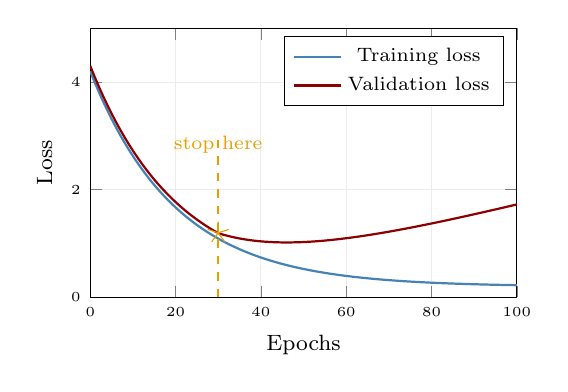
\begin{tikzpicture}
\begin{axis}[
    width=7cm, height=5cm,
    xlabel={Epochs}, ylabel={Loss},
    xlabel style={font=\footnotesize},
    ylabel style={font=\footnotesize},
    tick label style={font=\tiny},
    xmin=0, xmax=100, ymin=0, ymax=5,
    grid=major, grid style={gray!15},
    legend pos=north east,
    legend style={font=\scriptsize},
]
    % Training loss
    \addplot[thick, softblue, domain=0:100, samples=100]{4*exp(-0.05*x)+0.2};
    \addlegendentry{Training loss}
    % Validation loss
    \addplot[thick, darkred, domain=0:100, samples=100]{
        4*exp(-0.05*x) + 0.3 + 0.02*(x-30)*(x>30)
    };
    \addlegendentry{Validation loss}
    % Optimal point
    \draw[softorange, thick, dashed] (axis cs:30,0) -- (axis cs:30,3);
    \node[font=\scriptsize, softorange, above] at (axis cs:30,2.5) {stop here};
    \addplot[only marks, mark=star, mark size=4pt, softorange] coordinates {(30,1.2)};
\end{axis}
\end{tikzpicture}
\end{center}

\column{0.48\textwidth}
\vspace{0.3cm}
\textbf{Idea:} monitor the validation loss during training.  Stop when it starts increasing.

\vspace{0.3cm}
\textbf{In practice:}
\begin{enumerate}
    \item After each epoch, evaluate loss on validation set.
    \item Save model weights whenever validation loss improves.
    \item If no improvement for $p$ consecutive epochs (``patience''), stop training.
    \item Return the saved best weights.
\end{enumerate}

\vspace{0.3cm}
{\small Early stopping is a simple and effective form of regularization.}
\end{columns}
\end{frame}

% --- Slide 45: Regularization ---
\begin{frame}[shrink=10]{Regularization: $L_2$ Penalty and Dropout}
\begin{columns}[T]
\column{0.48\textwidth}
\textbf{$L_2$ Regularization (Weight Decay):}

Add a penalty to the loss:
\[
    \tilde{J}(\bm{\theta}) = J(\bm{\theta}) + \frac{\lambda}{2}\|\bm{\theta}\|_2^2
\]
Encourages small weights $\Rightarrow$ simpler model.

\vspace{0.2cm}
\textbf{Dropout} (Srivastava et al., 2014):

During training, randomly zero out each neuron with probability $p$ (typically 0.5). Forces the network not to rely on any single neuron. The standard \emph{inverted dropout} variant divides activations by $(1{-}p)$ during training, so no test-time rescaling is needed.

\column{0.48\textwidth}
\begin{center}
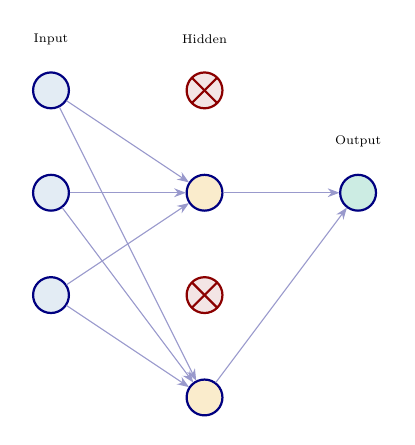
\begin{tikzpicture}[scale=0.65, transform shape,
    neuron/.style={circle, draw=uzhblue, thick, minimum size=7mm},
    dead/.style={circle, draw=darkred, thick, minimum size=7mm, fill=darkred!10,
                 path picture={\draw[darkred,thick] (path picture bounding box.south west)
                 -- (path picture bounding box.north east);
                 \draw[darkred,thick] (path picture bounding box.north west)
                 -- (path picture bounding box.south east);}},
    arr/.style={-{Stealth[length=1.5mm]}, uzhblue!40}]

    % Input
    \node[neuron, fill=softblue!15] (x1) at (0,2) {};
    \node[neuron, fill=softblue!15] (x2) at (0,0) {};
    \node[neuron, fill=softblue!15] (x3) at (0,-2) {};
    % Hidden
    \node[dead] (h1) at (3,2) {};
    \node[neuron, fill=softorange!20] (h2) at (3,0) {};
    \node[dead] (h3) at (3,-2) {};
    \node[neuron, fill=softorange!20] (h4) at (3,-4) {};
    % Output
    \node[neuron, fill=softgreen!20] (y) at (6,0) {};

    \foreach \i in {x1,x2,x3} {
        \draw[arr] (\i) -- (h2);
        \draw[arr] (\i) -- (h4);
    }
    \draw[arr] (h2) -- (y);
    \draw[arr] (h4) -- (y);

    \node[font=\scriptsize] at (0,3) {Input};
    \node[font=\scriptsize] at (3,3) {Hidden};
    \node[font=\scriptsize] at (6,1) {Output};
\end{tikzpicture}
\end{center}

\vspace{0.2cm}
{\small Dropout can be interpreted as training an \textbf{ensemble} of sub-networks that share weights.}
\end{columns}
\end{frame}

% --- Slide 47: Deep Double Descent ---
\begin{frame}[shrink=12]{Deep Double Descent}
\begin{columns}[T]
\column{0.52\textwidth}
\begin{center}
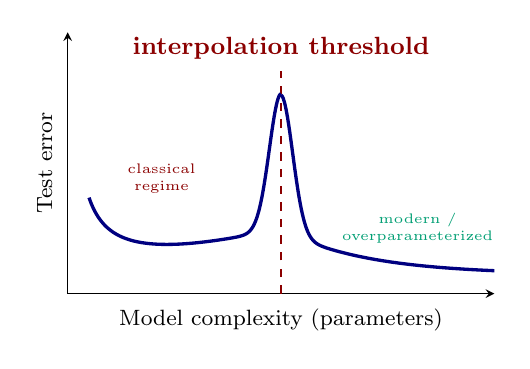
\begin{tikzpicture}
\begin{axis}[
    width=7cm, height=4.9cm,
    xlabel={Model complexity (parameters)},
    ylabel={Test error},
    xlabel style={font=\footnotesize},
    ylabel style={font=\footnotesize},
    tick label style={font=\tiny},
    xmin=0, xmax=10, ymin=0, ymax=6.8,
    grid=major, grid style={gray!15},
    xtick=\empty, ytick=\empty,
    axis lines=left,
    clip=false,
]
    % Interpolation threshold — vertical dashed marker + horizontal label above peak
    \draw[dashed, darkred, thick] (axis cs:5,0) -- (axis cs:5,5.8);
    \node[font=\small\bfseries, darkred, anchor=south]
        at (axis cs:5, 5.85) {interpolation threshold};

    % Single continuous curve: both pieces share the same spike,
    % so the two baselines match at x=5 (peak value ~5.17) and the
    % curve connects without a jump.
    % Classical regime + spike rise
    \addplot[very thick, uzhblue, domain=0.5:5, samples=200]
        {1.5/(x^0.7) + 0.15*(x^1.3) + 3.5*exp(-(x-5)^2/0.15)};
    % Modern regime + spike fall (identical spike term)
    \addplot[very thick, uzhblue, domain=5:10, samples=200]
        {0.5 + 1.17*exp(-0.5*(x-5)) + 3.5*exp(-(x-5)^2/0.15)};

    % Region labels
    \node[font=\tiny, darkred, align=center]
        at (axis cs:2.2, 3.0) {classical\\regime};
    \node[font=\tiny, softgreen, align=center]
        at (axis cs:8.2, 1.7) {modern /\\overparameterized};
\end{axis}
\end{tikzpicture}
\end{center}

\column{0.45\textwidth}
{\footnotesize The classical U turns into a \textbf{second descent} once the model is \emphc{overparameterized}. Three regimes along the curve:

\vspace{0.08cm}
\textcolor{darkred}{\textbf{1. Classical}} ($n_\text{par}\!<\!n_\text{data}$): the familiar bias--variance U --- small models underfit, larger ones chase noise.

\vspace{0.06cm}
\textcolor{darkred}{\textbf{2. Interpolation peak}} ($n_\text{par}\!\approx\!n_\text{data}$): model \emph{just} fits the training set; among all zero-error solutions the optimizer's pick is unstable $\Rightarrow$ variance explodes.

\vspace{0.06cm}
\textcolor{softgreen}{\textbf{3. Modern}} ($n_\text{par}\!\gg\!n_\text{data}$): gradient descent implicitly picks the \emphc{minimum-norm / smoothest} interpolator $\Rightarrow$ it generalizes \emph{better}. More parameters help.

\vspace{0.08cm}
{\scriptsize Belkin et al.\ (2019); Nakkiran et al.\ (2020).}}
\end{columns}

\vspace{0.05cm}
{\footnotesize\emphc{Hands-on:} \texttt{lectures/lecture\_02\_intro\_deep\_learning/code/lecture\_02\_03\_Double\_Descent.ipynb} --- reproduce the curve with random Fourier features.}
\end{frame}

% --- NTK / Benign Overfitting: further reading pointer ---
\begin{frame}{Further Reading: NTK and Benign Overfitting}
\begin{block}{Why does interpolation generalize? Two perspectives}
\begin{itemize}
    \item \textbf{Neural Tangent Kernel (NTK):} in the infinite-width limit, gradient descent on a neural network is equivalent to kernel regression with a fixed kernel; the kernel encodes the architecture.
    \begin{itemize}
        \item Jacot, Gabriel \& Hongler (2018, NeurIPS).
    \end{itemize}
    \item \textbf{Benign overfitting:} interpolators generalize when signal aligns with the top eigendirections and noise spreads across many small ones.
    \begin{itemize}
        \item Bartlett, Montanari \& Rakhlin (2021, \textit{Proc.\ Natl.\ Acad.\ Sci.}).
    \end{itemize}
\end{itemize}
\end{block}
\vspace{0.2cm}
{\footnotesize These theories provide a theoretical foundation for the double-descent phenomenon. Both are active research areas; consult the course reading list for entry points.}
\end{frame}

% ============================================================================
% PART 5.5: ADVANCED ARCHITECTURES & FRONTIERS
% ============================================================================

\section{Advanced Architectures \& Frontiers}

% --- Section Divider ---
\begin{frame}{}
\begin{center}
{\Huge \textcolor{uzhblue}{Part V}}\\[0.8em]
{\LARGE Advanced Architectures \& Frontiers}
\end{center}
\end{frame}

% --- Slide 48a: Reinforcement Learning in Finance (outlook only) ---
\begin{frame}{Outlook (not covered): RL in Finance}
\small
\begin{columns}[T]
\column{0.55\textwidth}
\textbf{The RL Loop:}
\begin{itemize}\itemsep1pt
    \item \textbf{Agent:} Portfolio manager / Algo trader
    \item \textbf{Environment:} The market (prices, order book)
    \item \textbf{State $s_t$:} Current prices, portfolio weights
    \item \textbf{Action $a_t$:} Buy/sell, rebalance
    \item \textbf{Reward $r_t$:} P\&L, Sharpe ratio, utility
\end{itemize}

\vspace{0.15cm}
\textbf{Why not in this course?}
\begin{itemize}\itemsep1pt
    \item RL finds \emph{strategies} in a \emph{fixed} environment.
    \item We focus on \emph{finding the equilibrium} (the environment itself).
    \item BUT: critical for hedging \& execution.
\end{itemize}

\column{0.42\textwidth}
\begin{center}
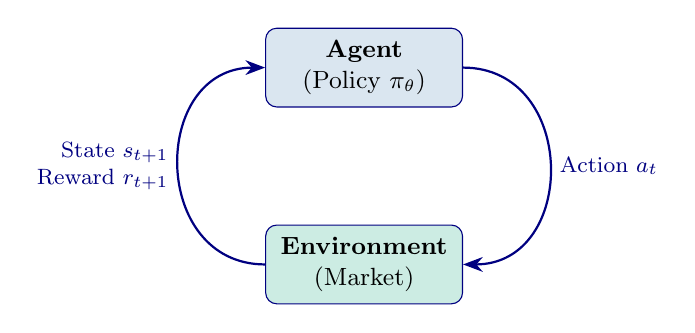
\begin{tikzpicture}[
    box/.style={rectangle, draw=uzhblue, fill=uzhgreylight, rounded corners=4pt,
                minimum width=2.5cm, minimum height=1cm, align=center, font=\small},
    arr/.style={-{Stealth[length=2.5mm]}, thick, uzhblue}
]
    \node[box, fill=softblue!20] (agent) at (0,2.5) {\textbf{Agent}\\(Policy $\pi_\theta$)};
    \node[box, fill=softgreen!20] (env) at (0,0) {\textbf{Environment}\\(Market)};

    \draw[arr] (agent.east) to[out=0,in=0,looseness=1.5] node[midway,right,font=\footnotesize] {Action $a_t$} (env.east);
    \draw[arr] (env.west) to[out=180,in=180,looseness=1.5] node[midway,left,font=\footnotesize,align=right] {State $s_{t+1}$\\Reward $r_{t+1}$} (agent.west);
\end{tikzpicture}
\end{center}
\end{columns}
\end{frame}

% ============================================================================
% Sequence Models mini-section: 9 slides building RNN → LSTM → Transformer
% ============================================================================

% --- Slide S1: Why sequences? ---
\begin{frame}{Why Sequences? Memory Matters}
\footnotesize
\textbf{Many real problems are intrinsically sequential:}
\begin{columns}[T]
\column{0.52\textwidth}
\begin{itemize}\itemsep1pt
    \item \emphc{Next-word prediction:} ``Today we are having a class on deep \rule{0.9cm}{0.4pt}''
    \item \emphc{Time-series forecasting:} inflation, volatility, returns conditional on history
    \item \emphc{Audio / music:} each sample predicted from thousands before (MuseNet, Wav2Vec)
    \item \emphc{Econ application:} Edgeworth cycles in gasoline prices (asymmetric sawtooth)
\end{itemize}

\column{0.46\textwidth}
\textbf{Why an MLP is not enough.}
\begin{itemize}\itemsep1pt
    \item MLP output is \emph{memoryless}: $\hat{y}_t = f(\x_t)$.
    \item Same input $\Rightarrow$ same output, regardless of history.
    \item Sequences have \emph{variable length}; MLPs have a fixed input size.
    \item We need a network that \emphc{carries state across time}.
\end{itemize}
\end{columns}

\vspace{5pt}
\begin{center}
\small
\emphc{Design goals} (Elman 1990; Rumelhart, Hinton \& Williams 1986): \textbf{variable length} $\cdot$ \textbf{order} $\cdot$ \textbf{long-range dependence} $\cdot$ \textbf{parameter sharing across time}.
\end{center}
\end{frame}

% --- Slide S2: From MLP to Recurrence ---
\begin{frame}{From MLP to Recurrence}
\footnotesize
\textbf{Idea.} Give the cell a persistent \emphc{hidden state} $\bm{h}_t \in \R^d$, fed back at every step.

\vspace{2pt}
\begin{columns}[T]
\column{0.55\textwidth}
\begin{itemize}\itemsep1pt
    \item At step $t$, the cell sees \emph{both} the new input $\x_t$ and yesterday's state $\bm{h}_{t-1}$.
    \item Same parameters $\{\W_{hh},\W_{xh},\bb\}$ at every step: \emphc{parameter sharing across time}.
    \item The hidden state $\bm{h}_t$ is a learned summary of the past, the network's ``memory''.
    \item \emph{One} cell processes \emph{any} sequence length.
\end{itemize}

\vspace{3pt}
\begin{center}
{\scriptsize \emphc{RNN is a dynamical system.}  Not a static function.}
\end{center}

\column{0.44\textwidth}
\centering
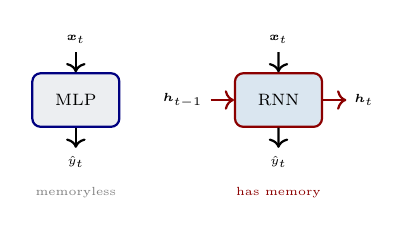
\begin{tikzpicture}[scale=0.85, transform shape, font=\scriptsize,
    m/.style={rectangle, draw=uzhblue, thick, rounded corners=3pt, fill=uzhgreylight,
              minimum width=1.3cm, minimum height=0.8cm, align=center},
    r/.style={rectangle, draw=darkred, thick, rounded corners=3pt, fill=softblue!20,
              minimum width=1.3cm, minimum height=0.8cm, align=center}]
% MLP
\node[m] (mlp) at (0,0) {MLP};
\node[above=0.3cm of mlp, font=\tiny] (xm) {$\x_t$};
\node[below=0.3cm of mlp, font=\tiny] (ym) {$\hat{y}_t$};
\draw[->,thick] (xm) -- (mlp);
\draw[->,thick] (mlp) -- (ym);
\node[below=0.05cm of ym, font=\tiny, gray] {memoryless};

% RNN
\node[r, right=1.7cm of mlp] (rnn) {RNN};
\node[above=0.3cm of rnn, font=\tiny] (xr) {$\x_t$};
\node[below=0.3cm of rnn, font=\tiny] (yr) {$\hat{y}_t$};
\draw[->,thick] (xr) -- (rnn);
\draw[->,thick] (rnn) -- (yr);
\node[font=\tiny, left=0.35cm of rnn] (hin) {$\bm{h}_{t-1}$};
\draw[->,thick,darkred] (hin) -- (rnn);
\node[font=\tiny, right=0.35cm of rnn] (hout) {$\bm{h}_t$};
\draw[->,thick,darkred] (rnn) -- (hout);
\node[below=0.05cm of yr, font=\tiny, darkred] {has memory};
\end{tikzpicture}
\end{columns}
\end{frame}

% --- Slide S3: The RNN cell, unrolled ---
\begin{frame}{The RNN Cell, Unrolled Across Time}
\footnotesize
\begin{columns}[T]
\column{0.44\textwidth}
\textbf{Two equations} define the cell:
\[
\boxed{\;\bm{h}_t = \tanh\!\big(\W_{hh}\,\bm{h}_{t-1} + \W_{xh}\,\x_t + \bb_h\big)\;}
\]
\[
\hat{y}_t = \W_{hy}\,\bm{h}_t + \bb_y
\]

\vspace{4pt}
\begin{itemize}\itemsep1pt
    \item $\bm{h}_0$ initialized to $\bm{0}$ (or learned).
    \item \emphc{Weight sharing:} $\W_{hh},\W_{xh},\W_{hy}$ do not depend on $t$.
    \item A \emph{folded} loop with $T$ steps $\equiv$ an \emph{unfolded} feedforward graph of depth $T$ with \emph{shared} parameters.
\end{itemize}

\column{0.55\textwidth}
\centering
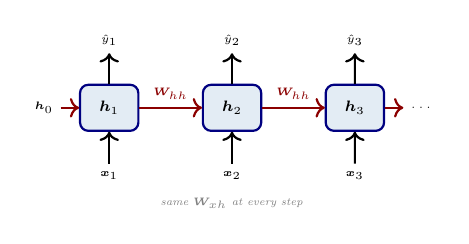
\begin{tikzpicture}[scale=0.78, transform shape, font=\scriptsize,
    c/.style={rectangle, draw=uzhblue, thick, rounded corners=3pt, fill=softblue!15,
              minimum width=0.95cm, minimum height=0.75cm, align=center}]
\foreach \t/\xpos in {1/0, 2/2, 3/4} {
    \node[c] (h\t) at (\xpos,0) {$\bm{h}_\t$};
    \node[font=\tiny] (x\t) at (\xpos,-1.1) {$\x_\t$};
    \node[font=\tiny] (y\t) at (\xpos, 1.1) {$\hat{y}_\t$};
    \draw[->,thick] (x\t) -- (h\t);
    \draw[->,thick] (h\t) -- (y\t);
}
\node[font=\tiny, left=0.3cm of h1] (h0) {$\bm{h}_0$};
\draw[->,thick,darkred] (h0) -- (h1);
\draw[->,thick,darkred] (h1) -- node[above,font=\tiny]{$\W_{hh}$} (h2);
\draw[->,thick,darkred] (h2) -- node[above,font=\tiny]{$\W_{hh}$} (h3);
\node[font=\tiny, right=0.3cm of h3] (hN) {$\cdots$};
\draw[->,thick,darkred] (h3) -- (hN);
\node[font=\tiny, below=0.05cm of x2, gray] {\emph{same $\W_{xh}$ at every step}};
\end{tikzpicture}
\vspace{3pt}
\\
{\scriptsize\emphc{``Same function, many steps.''} Elman (1990); Rumelhart, Hinton \& Williams (1986).}
\end{columns}
\end{frame}

% --- Slide S4: BPTT + vanishing/exploding ---
\begin{frame}[shrink=10]{Training: Backpropagation Through Time (BPTT)}
\footnotesize
\textbf{Idea.}  The unrolled RNN is a feedforward net of depth $T$ with \emph{shared} weights.  Run backprop, \emph{sum} weight-gradients across time.

\vspace{3pt}
\begin{columns}[T]
\column{0.56\textwidth}
\textbf{Gradient through time.} For the gradient of $\mathcal{L}_T$ w.r.t.\ an early state $\bm{h}_k$,
\[
\nabla_{\bm{h}_k}\mathcal{L}_T \;=\; \Bigl(\!\prod_{t=k+1}^{T} \underbrace{\frac{\partial \bm{h}_t}{\partial \bm{h}_{t-1}}}_{=\,\mathrm{diag}(\tanh')\,\W_{hh}}\!\Bigr)^{\!\!\top}\,\nabla_{\bm{h}_T}\mathcal{L}_T.
\]
{\scriptsize Standard Jacobian convention; the transpose rides on the chain-rule product. Details in the script's \S1.10 ``Vanishing and Exploding Gradients''.}\\[1pt]
A \emphc{long product of the same Jacobian}:
\begin{itemize}\itemsep0pt
    \item If $\|\W_{hh}\|\!>\!1$: gradient \emphc{explodes} $\to$ NaN.
    \item If $\|\W_{hh}\|\!<\!1$: gradient \emphc{vanishes} $\to$ no learning of long-range structure.
\end{itemize}

\vspace{1pt}
{\scriptsize\emphc{Remedies:} gradient clipping, orthogonal init, truncated BPTT, and above all \emphc{gated cells} (LSTM, GRU).}

\column{0.42\textwidth}
\centering
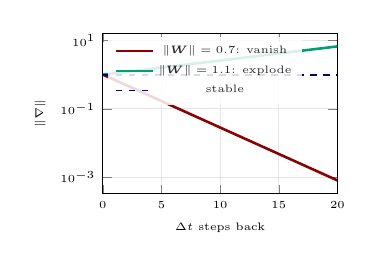
\begin{tikzpicture}[scale=0.78, transform shape, font=\scriptsize]
\begin{axis}[
    width=5.4cm, height=4.2cm,
    xlabel={$\Delta t$ steps back}, ylabel={$\|\nabla\|$},
    xlabel style={font=\tiny}, ylabel style={font=\tiny},
    tick label style={font=\tiny}, ymode=log,
    domain=0:20, samples=40, xmin=0, xmax=20,
    legend style={font=\tiny, at={(0.02,0.98)}, anchor=north west,
                  draw=none, fill=white, fill opacity=0.85},
    grid=both, grid style={gray!20}]
\addplot[darkred, very thick] {0.7^x};
\addlegendentry{$\|\W\|=0.7$: vanish}
\addplot[softgreen, very thick] {1.1^x};
\addlegendentry{$\|\W\|=1.1$: explode}
\addplot[uzhblue, thick, dashed] {1};
\addlegendentry{stable}
\end{axis}
\end{tikzpicture}
\end{columns}
\end{frame}

% --- Slide S5: LSTM ---
\begin{frame}[shrink=8]{LSTM: A Memory Conveyor Belt}
\footnotesize
\textbf{Plain-language picture.} A vanilla RNN rewrites its memory at every step.  An LSTM keeps a dedicated \emphc{cell state} $\bm{C}_t$ that mostly flows forward unchanged.

\vspace{2pt}
\begin{columns}[T]
\column{0.54\textwidth}
\textbf{At each date, the cell makes three soft decisions:}
\begin{itemize}\itemsep1pt
    \item \emphc{Forget gate} $f_t$: how much of the old memory survives?
    \item \emphc{Input gate} $i_t$: how much new information should be written?
    \item \emphc{Output gate} $o_t$: how much of memory should be exposed as $\bm{h}_t$?
\end{itemize}

\vspace{2pt}
\[
\bm{C}_t = \bm{f}_t \odot \bm{C}_{t-1} + \bm{i}_t \odot \tilde{\bm{C}}_t,
\qquad
\bm{h}_t = \bm{o}_t \odot \tanh(\bm{C}_t)
\]

\vspace{1pt}
\begin{itemize}\itemsep1pt
    \item \emphc{Key win:} memory changes \emph{additively}, so useful information can survive many steps.
    \item Useful for persistent asymmetric patterns, e.g.\ Edgeworth cycles.
\end{itemize}

\column{0.45\textwidth}
\centering
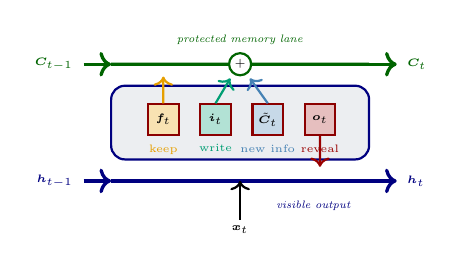
\begin{tikzpicture}[scale=0.78, transform shape, font=\scriptsize,
    cell/.style={rectangle, draw=uzhblue, thick, rounded corners=5pt, fill=uzhgreylight,
                 minimum width=4.2cm, minimum height=1.2cm},
    g/.style={rectangle, draw=darkred, thick, fill=red!10,
              minimum size=0.5cm, font=\tiny, inner sep=1pt},
    plus/.style={circle, draw=darkgreen, thick, fill=white,
                 minimum size=0.36cm, inner sep=0pt, font=\tiny}]
% top lane label — well above the C labels
\node[font=\tiny,darkgreen] at (0,1.35) {\emph{protected memory lane}};
% cell box
\node[cell] (c) at (0,0) {};
% gates centered inside the cell
\node[g, fill=softorange!30] (f) at (-1.25,0.05) {$\bm{f}_t$};
\node[g, fill=softgreen!30]  (i) at (-0.40,0.05) {$\bm{i}_t$};
\node[g, fill=softblue!30]   (u) at ( 0.45,0.05) {$\tilde{\bm{C}}_t$};
\node[g, fill=harvardcrimson!25] (o) at ( 1.30,0.05) {$\bm{o}_t$};
\node[plus] (add) at (0.0,0.95) {$+$};
% Cell-state top lane; C labels inline at the ends
\draw[->, very thick, darkgreen] (-2.55, 0.95) -- (-2.1, 0.95);
\draw[very thick, darkgreen] (-2.1, 0.95) -- (add.west);
\draw[very thick, darkgreen] (add.east) -- (2.1, 0.95);
\draw[->, very thick, darkgreen] (2.1, 0.95) -- (2.55, 0.95);
\node[darkgreen, font=\tiny, anchor=east] at (-2.60, 0.95) {$\bm{C}_{t-1}$};
\node[darkgreen, font=\tiny, anchor=west] at ( 2.60, 0.95) {$\bm{C}_t$};
% Hidden lane; h labels inline at the ends
\draw[->, very thick, uzhblue] (-2.55, -0.95) -- (-2.1, -0.95);
\draw[very thick, uzhblue] (-2.1, -0.95) -- (2.1, -0.95);
\draw[->, very thick, uzhblue] (2.1, -0.95) -- (2.55, -0.95);
\node[uzhblue, font=\tiny, anchor=east] at (-2.60, -0.95) {$\bm{h}_{t-1}$};
\node[uzhblue, font=\tiny, anchor=west] at ( 2.60, -0.95) {$\bm{h}_t$};
% bottom lane label — offset right so it does not clash with the x_t arrow at x=0
\node[font=\tiny,uzhblue] at (1.2,-1.35) {\emph{visible output}};
% gate internal arrows
\draw[->, thick, softorange] (f.north) -- (-1.25,0.75);
\draw[->, thick, softgreen] (i.north) -- (-0.16,0.72);
\draw[->, thick, softblue] (u.north) -- (0.16,0.72);
\draw[->, thick, harvardcrimson] (o.south) -- (1.30,-0.72);
\node[below=0.02cm of f, font=\tiny, softorange] {keep};
\node[below=0.02cm of i, font=\tiny, softgreen] {write};
\node[below=0.02cm of u, font=\tiny, softblue] {new info};
\node[below=0.02cm of o, font=\tiny, harvardcrimson] {reveal};
% x input — enters vertically from below the cell
\node[font=\tiny] at (0,-1.75) {$\x_t$};
\draw[->, thick] (0,-1.58) -- (0,-0.95);
\end{tikzpicture}
\end{columns}

\end{frame}

% --- Slide S6: Limits of recurrence → attention ---
\begin{frame}{Limits of Recurrence $\Rightarrow$ Attention}
\footnotesize
\textbf{Even with LSTMs, two hard limits remain.}

\vspace{3pt}
\begin{columns}[T]
\column{0.5\textwidth}
\textcolor{darkred}{\textbf{1. Sequential $\Rightarrow$ no parallelism.}}
\begin{itemize}\itemsep0pt
    \item Step $t$ must wait for step $t{-}1$.
    \item GPUs love parallelism $\Rightarrow$ RNN training is memory-bound and slow.
    \item Training modern LLMs on $\sim$\,1T tokens with RNNs would take \emph{years}.
\end{itemize}

\column{0.5\textwidth}
\textcolor{darkred}{\textbf{2. Path length blurs long-range signals.}}
\begin{itemize}\itemsep0pt
    \item Information from position 1 reaches position $T$ through $T{-}1$ hops.
    \item Each hop applies a matrix + nonlinearity $\Rightarrow$ fading memory.
    \item Gating helps but does not eliminate path-length decay.
\end{itemize}
\end{columns}

\vspace{6pt}
\begin{center}
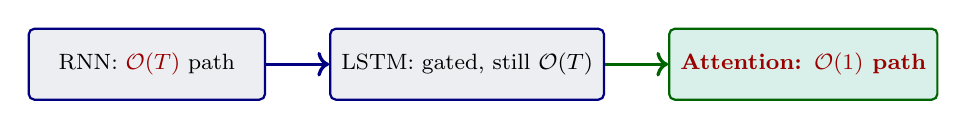
\begin{tikzpicture}[font=\footnotesize,
    b/.style={draw=uzhblue,thick,rounded corners=2pt,fill=uzhgreylight,
              inner sep=4pt,minimum height=9mm,minimum width=30mm,align=center}]
\node[b] (rnn) {RNN: \emphc{$\mathcal{O}(T)$} path};
\node[b,right=8mm of rnn] (lstm) {LSTM: gated, still $\mathcal{O}(T)$};
\node[b,right=8mm of lstm, fill=softgreen!15, draw=darkgreen] (att) {\emphc{\textbf{Attention: $\mathcal{O}(1)$ path}}};
\draw[->,very thick,uzhblue] (rnn) -- (lstm);
\draw[->,very thick,darkgreen] (lstm) -- (att);
\end{tikzpicture}
\end{center}

\vspace{2pt}
{\scriptsize\emphc{Key move.}  Drop recurrence entirely: let every position read every other \emph{directly}, in \emph{parallel}.  This is the \emphc{Transformer} (Vaswani et al.\ 2017).}
\end{frame}

% --- Slide S7: Self-attention intuition ---
\begin{frame}{Self-Attention: Search Inside the Sequence}
\footnotesize
\begin{columns}[T]
\column{0.46\textwidth}
\textbf{Mental model.} Updating a token is a search over the whole sequence.

\vspace{0.04cm}
\textbf{Each token creates three vectors:}
\begin{itemize}\itemsep0pt
    \item[\textcolor{softblue}{$\blacktriangleright$}] \textcolor{softblue}{\textbf{Query $q_i$}}: what am I looking for?
    \item[\textcolor{harvardcrimson}{$\blacktriangleright$}] \textcolor{harvardcrimson}{\textbf{Key $k_j$}}: what does token $j$ advertise?
    \item[\textcolor{softgreen}{$\blacktriangleright$}] \textcolor{softgreen}{\textbf{Value $v_j$}}: what can token $j$ contribute?
\end{itemize}

\vspace{0.04cm}
\textbf{Four-step recipe:}
\begin{enumerate}\itemsep0pt
    \item Add position information.
    \item Compare $q_i$ with every key $k_j$.
    \item Softmax the scores into weights $\alpha_{ij}$.
    \item Return the weighted average of the values.
\end{enumerate}

\column{0.52\textwidth}
\centering
{\small\textbf{Worked attention pattern}}

\vspace{0.05cm}
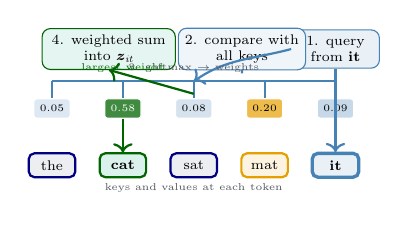
\begin{tikzpicture}[scale=0.72, transform shape, font=\scriptsize,
    tok/.style={rectangle, draw=uzhblue, thick, rounded corners=2pt, fill=uzhgreylight,
                minimum width=0.82cm, minimum height=0.42cm, inner sep=1pt},
    wt/.style={rectangle, draw=white, rounded corners=1pt, minimum width=0.64cm,
               minimum height=0.34cm, inner sep=1pt, font=\tiny},
    box/.style={rounded corners=3pt, align=center},
    lab/.style={font=\tiny, text=uzhgreydark}]
\node[tok] (t1) at (0.0,0.0) {the};
\node[tok, fill=softgreen!14, draw=darkgreen] (t2) at (1.25,0.0) {\textbf{cat}};
\node[tok] (t3) at (2.50,0.0) {sat};
\node[tok, fill=softorange!12, draw=softorange] (t4) at (3.75,0.0) {mat};
\node[tok, fill=softblue!12, draw=softblue, very thick] (t5) at (5.00,0.0) {\textbf{it}};
\node[wt, fill=softblue!18] (w1) at (0.0,1.0) {0.05};
\node[wt, fill=darkgreen!75, text=white] (w2) at (1.25,1.0) {0.58};
\node[wt, fill=softblue!22] (w3) at (2.50,1.0) {0.08};
\node[wt, fill=softorange!70] (w4) at (3.75,1.0) {0.20};
\node[wt, fill=softblue!30] (w5) at (5.00,1.0) {0.09};
\node[draw=softblue, fill=softblue!12, box,
      minimum width=1.55cm, minimum height=0.56cm] (q) at (5.00,2.05) {1. query\\from \textbf{it}};
\node[draw=softblue, fill=softblue!8, box,
      minimum width=1.9cm, minimum height=0.52cm] (cmp) at (3.35,2.05) {2. compare with\\all keys};
\node[draw=darkgreen, fill=softgreen!10, box,
      minimum width=2.35cm, minimum height=0.60cm] (z) at (1.00,2.05)
      {4. weighted sum\\into $\bm{z}_{\textit{it}}$};
\draw[->, thick, softblue] (q.south) -- (t5.north);
\draw[softblue, thick] (0.0,1.48) -- (5.00,1.48);
\foreach \x in {0.0,1.25,2.50,3.75,5.00} {
    \draw[softblue, thick] (\x,1.48) -- (\x,1.18);
}
\draw[->, thick, softblue] (q.west) to[out=195,in=35] (2.50,1.48);
\draw[softblue, thick] (cmp.south) -- (3.35,1.62);
\draw[->, thick, darkgreen] (2.50,1.26) -- (z.south);
\draw[->, thick, darkgreen] (w2.south) -- (t2.north);
\node[lab] at (2.50,1.72) {3. softmax $\rightarrow$ weights};
\node[lab] at (2.50,-0.40) {keys and values at each token};
\node[font=\tiny, darkgreen] at (1.25,1.72) {largest weight};
\end{tikzpicture}

\vspace{0.04cm}
{\scriptsize Blue arrows: build the query and compare it to all keys.  Green arrows: use the weights to pull information, mainly from ``cat'', into $\bm{z}_{\textit{it}}$.}
\\[-1pt]
{\scriptsize Displayed weights: $0.05 + 0.58 + 0.08 + 0.20 + 0.09 = 1.00$.}
\end{columns}
\end{frame}

% --- Slide S8: Transformer block ---
\begin{frame}{From Self-Attention to a Transformer Block}
\footnotesize
\begin{columns}[T]
\column{0.48\textwidth}
\textbf{Matrix form:}
\[
\mathrm{Attn}(Q,K,V) =
\mathrm{softmax}\!\left(\frac{QK^\top}{\sqrt{d_k}}\right)V
\]

\vspace{2pt}
\textbf{Why the extra ingredients?}
\begin{itemize}\itemsep1pt
    \item \textbf{Multi-head attention:} different heads can focus on different relations in parallel.
    \item \textbf{Positional encoding:} attention alone cannot see order, so we add a ruler.
    \item \textbf{Residuals + LayerNorm + MLP:} make deep stacks trainable and expressive.
\end{itemize}
\vspace{2pt}
{\scriptsize\emphc{Econ gloss:} learnable kernel smoothing with learned features and learned similarity.}

\column{0.50\textwidth}
\centering
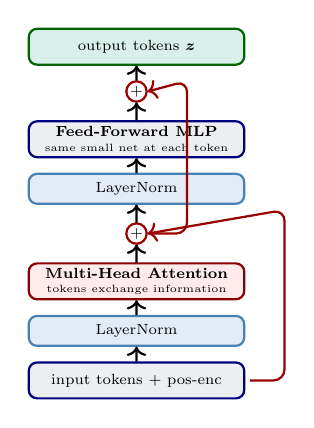
\begin{tikzpicture}[scale=0.76, transform shape, font=\scriptsize,
    b/.style={draw=uzhblue, thick, rounded corners=3pt, fill=uzhgreylight,
              minimum width=3.6cm, minimum height=0.6cm, inner sep=2pt, align=center},
    attn/.style={draw=darkred, thick, rounded corners=3pt, fill=red!8,
              minimum width=3.6cm, minimum height=0.6cm, inner sep=2pt, align=center},
    ln/.style={draw=softblue, thick, rounded corners=3pt, fill=softblue!15,
              minimum width=3.6cm, minimum height=0.5cm, inner sep=2pt, align=center},
    plus/.style={circle, draw=harvardcrimson, thick, fill=white,
                 minimum size=0.34cm, inner sep=0pt, font=\scriptsize}]
\node[b] (in) at (0,0) {input tokens $+$ pos-enc};
\node[ln, above=0.25cm of in] (ln1) {LayerNorm};
\node[attn, above=0.25cm of ln1] (mha) {\textbf{Multi-Head Attention}\\[-1pt]{\tiny tokens exchange information}};
\node[plus, above=0.30cm of mha] (add1) {$+$};
\node[ln, above=0.30cm of add1] (ln2) {LayerNorm};
\node[b, above=0.25cm of ln2] (ff) {\textbf{Feed-Forward MLP}\\[-1pt]{\tiny same small net at each token}};
\node[plus, above=0.30cm of ff] (add2) {$+$};
\node[b, above=0.25cm of add2, fill=softgreen!15, draw=darkgreen] (out) {output tokens $\bm{z}$};
\draw[->,thick] (in) -- (ln1);
\draw[->,thick] (ln1) -- (mha);
\draw[->,thick] (mha) -- (add1);
\draw[->,thick] (add1) -- (ln2);
\draw[->,thick] (ln2) -- (ff);
\draw[->,thick] (ff) -- (add2);
\draw[->,thick] (add2) -- (out);
\draw[->, thick, harvardcrimson, rounded corners=4pt]
    ($(in.east)+(0.08,0)$) -- ++(0.58,0) -- ++(0,2.85) -- (add1.east);
\draw[->, thick, harvardcrimson, rounded corners=4pt]
    ($(add1.east)+(0.08,0)$) -- ++(0.58,0) -- ++(0,2.55) -- (add2.east);
\end{tikzpicture}
\\[1pt]
{\scriptsize\emphc{One block} first mixes information \emph{across tokens}, then transforms each token with an MLP, while skip connections keep deep stacks trainable.}
\end{columns}
\end{frame}

% --- Slide S9: practical takeaway ---
\begin{frame}{RNN, LSTM, Transformer: What to Remember}
\footnotesize
\begin{columns}[T]
\column{0.32\textwidth}
\begin{block}{RNN}
\begin{itemize}\itemsep1pt
    \item Hidden state = running summary of the past
    \item Best first mental model for sequence learning
    \item Hard to train on long histories
\end{itemize}
\end{block}

\column{0.32\textwidth}
\begin{block}{LSTM / GRU}
\begin{itemize}\itemsep1pt
    \item Add gates and a protected memory lane
    \item Strong baseline for specialized time-series tasks
    \item Still sequential, so no large-scale parallelism
\end{itemize}
\end{block}

\column{0.32\textwidth}
\begin{block}{Transformer}
\begin{itemize}\itemsep1pt
    \item Every token can read every other token directly
    \item Full parallelism across positions
    \item Default choice for long-context sequence modeling
\end{itemize}
\end{block}
\end{columns}

\vspace{3pt}
\begin{exampleblock}{Rule of Thumb}
If the pattern is specialized and the history is moderate, an LSTM is still a strong baseline.  If context is long and parallelism matters, start with a Transformer.
\end{exampleblock}

\vspace{1pt}
{\scriptsize Earlier-lecture notebooks: \texttt{08\_MLP\_LSTM\_Transformer\_Edgeworth\_Cycles} (the three-way comparison on the same task) and \texttt{09\_Transformer\_InContext\_AR1} (advanced / optional).}
\end{frame}

% ============================================================================
% PART 6: PRACTICE AND EXERCISES
% ============================================================================

\section{Practice and Exercises}

% --- Section Divider ---
\begin{frame}{}
\begin{center}
{\Huge \textcolor{uzhblue}{Part VI}}\\[0.8em]
{\LARGE Software, Exercises, and Next Steps}
\end{center}
\end{frame}

% --- Slide 49: Software Ecosystem ---
\begin{frame}[shrink=8]{Software Ecosystem}
\begin{center}

\begin{tikzpicture}[
    fw/.style={rectangle, draw=uzhblue, fill=uzhblue!8, rounded corners=5pt,
               minimum width=3.2cm, minimum height=1.5cm, align=center, font=\small}
]
    \node[fw, fill=softorange!15] (tf) at (0,0) {\textbf{\large TensorFlow}\\+ Keras\\{\scriptsize Google, 2015}};
    \node[fw, fill=darkred!8] (pt) at (5.5,0) {\textbf{\large PyTorch}\\{\scriptsize Meta AI, 2017}};
    \node[fw, fill=softgreen!10] (jax) at (11,0) {\textbf{\large JAX}\\{\scriptsize Google, 2018}};
\end{tikzpicture}
\end{center}

\vspace{0.3cm}
\begin{itemize}
    \item \textbf{Keras} (\url{https://keras.io}) provides a high-level API that runs on top of TensorFlow, PyTorch, or JAX---write once, run anywhere.
    \item \textbf{Key resources:}
    \begin{itemize}
        \item Keras sequential model: \url{https://www.tensorflow.org/guide/keras/sequential_model}
        \item TensorBoard: \url{https://www.tensorflow.org/tensorboard}
        \item PyTorch tutorials: \url{https://pytorch.org/tutorials}
    \end{itemize}
\end{itemize}

\vspace{0.2cm}
{\footnotesize\emphc{This chapter exercises both stacks:} notebooks 04, 05, 07 use \emphc{TensorFlow/Keras}; notebooks 06, 08, 09 use \emphc{PyTorch}. Later DEQN/PINN material is TensorFlow-based; the heterogeneous-agent and sequence-space chapters add JAX.}
\end{frame}

% --- Slide 49b: Notation pact ---
\begin{frame}{Notation Pact for the Rest of the Course}
\footnotesize
This chapter uses $\bm{\theta}$ for generic trainable model parameters, following the textbook convention.  From Chapter~2 onward the script switches:
\vspace{0.3em}
\begin{itemize}\itemsep2pt
    \item $\rho$ = neural-network weights (e.g.\ $\mathcal{N}_\rho(\x)$), matching Azinovic, Gaegauf \& Scheidegger (2022) and the rest of the DEQN literature.
    \item $\bm{\theta}$ = \emph{structural} economic parameters that the network does not see (e.g.\ Chs.~10 \& 11 on structural estimation and climate).
\end{itemize}
\vspace{0.4em}
Both symbols denote the same object \emph{abstractly} (free parameters of the model); the rename foregrounds which kind of parameter is being trained.  Whenever a network appears in subsequent chapters, expect $\rho$.
\end{frame}

% --- Slide 50: Hands-on Notebooks ---
\begin{frame}[shrink=15]{Hands-On Notebooks}
The companion Jupyter notebooks are available in the course repository:

\vspace{0.3cm}
\begin{center}
{\scriptsize
\renewcommand{\arraystretch}{1.15}
\begin{tabular}{clp{5.2cm}}
\toprule
\textbf{\#} & \textbf{Notebook} & \textbf{Content} \\
\midrule
1 & \texttt{01\_BasicML\_intro} & Linear regression, classification, clustering, loss functions \\
2 & \texttt{02\_GradientDescent\_and\_SGD} & Gradient descent, line search, SGD \\
3 & \texttt{03\_Double\_Descent} & Double-descent with random Fourier features \\
4 & \texttt{04\_Gentle\_DNN} & First neural network with Keras \\
5 & \texttt{05\_Tensorboard} & Visualizing training with TensorBoard \\
6 & \texttt{06\_PyTorch\_intro} & Introduction to PyTorch \\
7 & \texttt{07\_Genz\_Approximation\_and\_Loss} & Genz functions, NN approximation, robust losses \\
8 & \texttt{08\_MLP\_LSTM\_Transformer\_Edgeworth\_Cycles} & MLP vs LSTM vs tiny Transformer on Edgeworth cycles \\
9 & \texttt{09\_Transformer\_InContext\_AR1} & Tiny transformer, in-context learning of AR(1) \\
\bottomrule
\end{tabular}
\vspace{0.2cm}\\
{\tiny File \#2: \texttt{02\_GradientDescent\_and\_StochasticGradientDescent.ipynb};\ \#7: \texttt{07\_Genz\_Approximation\_and\_Loss\_Functions.ipynb}.}
}%
\end{center}
\end{frame}

% --- Slide 51: Exercise 1 ---
\begin{frame}[shrink=12]{Exercise: Function Approximation with Neural Networks}
\textbf{Task:} approximate the Genz (1987) test functions with neural networks.

\vspace{0.2cm}
\begin{footnotesize}
\begin{align*}
    f_1(\x) &= \cos\!\Big(2\pi w_1 + \textstyle\sum_{i=1}^{d} c_i x_i\Big) & &\text{(oscillatory)} \\
    f_2(\x) &= \textstyle\prod_{i=1}^{d} \big(c_i^{-2} + (x_i - w_i)^2\big)^{-1} & &\text{(product peak)} \\
    f_3(\x) &= \Big(1 + \textstyle\sum_{i=1}^{d} c_i x_i\Big)^{-(d+1)} & &\text{(corner peak)} \\
    f_4(\x) &= \exp\!\Big(-\textstyle\sum_{i=1}^{d} c_i^2(x_i - w_i)^2\Big) & &\text{(Gaussian)} \\
    f_5(\x) &= \exp\!\Big(-\textstyle\sum_{i=1}^{d} c_i|x_i - w_i|\Big) & &\text{(continuous)} \\
    f_6(\x) &= \begin{cases}0 & \text{if } x_1>w_1 \text{ or } x_2>w_2\\ \exp\!\big(\textstyle\sum_{i=1}^{d}c_i x_i\big) & \text{otherwise}\end{cases} & &\text{(discontinuous)}
\end{align*}
\end{footnotesize}

\vspace{0.1cm}
{\small Pick 3 functions. Train NNs on 10, 50, 100, 500 random points from $[0,1]^d$.  Compute average and max error on 1000 test points.  Repeat for $d\in\{2,5,10\}$.}
\end{frame}

% --- Slide 52: Exercise 2 ---
\begin{frame}{Exercise: Architecture Exploration}
\textbf{Using the Genz functions from the previous exercise:}

\vspace{0.4cm}
\begin{enumerate}
    \item \textbf{Vary the depth:} try 1, 2, 3, and 5 hidden layers.  How does depth affect approximation quality?

    \vspace{0.3cm}
    \item \textbf{Vary the activation:} compare sigmoid, tanh, ReLU, and Swish.  Which works best for smooth vs.\ discontinuous functions?

    \vspace{0.3cm}
    \item \textbf{Vary the optimizer:} compare plain SGD, SGD with momentum, and Adam.  Monitor convergence speed and final accuracy.

    \vspace{0.3cm}
    \item \textbf{Plot} the maximum and average approximation error as a function of the number of training points.  What happens as $d$ grows?
\end{enumerate}

\vspace{0.3cm}
{\small \textbf{Hint:} you should observe the ``curse of dimensionality'', the error grows significantly with $d$ for a fixed number of training points.}
\end{frame}

% --- Slide 53: Questions ---
\begin{frame}{}
\begin{columns}[c]
\column{0.45\textwidth}
\begin{center}
\includegraphics[width=0.85\textwidth]{figures/quest.png}
\end{center}

\column{0.50\textwidth}
\begin{center}
{\Huge \textcolor{uzhblue}{\textbf{Questions?}}}

\vspace{0.8cm}
{\large Simon Scheidegger}\\[4pt]
{\small HEC, University of Lausanne}\\[4pt]
\url{https://sischei.github.io}

\vspace{0.6cm}
{\small Materials:~~\url{https://github.com/sischei/Deep_Learning_for_Solving_And_Estimating_Dynamic_Economic_Models}}
\end{center}
\end{columns}
\end{frame}

\end{document}
